%--------------------------------------------------------------
%   AUTH: David Chalco
%   DESC: Lab template
%   DATE: 01-16-2017
%-------------------------------------------------------------
\documentclass[12pt,a4paper]{article}
\usepackage[utf8]{inputenc}
\usepackage{graphicx}
\usepackage{amsmath}
\usepackage{amssymb}
\usepackage{bm}
\usepackage{mathtools}
\usepackage{ragged2e}
\usepackage{epstopdf}
\usepackage{multicol}
\usepackage[siunitx,european,american]{circuitikz}
\usepackage{subcaption}
\usepackage{paracol}
\usepackage{enumitem}
\usepackage{mwe}
\usepackage{chemstyle}
\usepackage[version=3]{mhchem}
\usepackage{amsfonts}
\usepackage{textcomp}
\usepackage{pdfpages}
\usepackage{caption}
\usepackage{tikz} 
\usepackage{listings}
\usepackage{color}
\definecolor{codegreen}{rgb}{0,0.6,0}
\definecolor{codegray}{rgb}{0.5,0.5,0.5}
\definecolor{codepurple}{rgb}{0.58,0,0.82}
\definecolor{backcolour}{rgb}{0.95,0.95,0.92}
\usetikzlibrary{fit}

\lstdefinelanguage[Objective]{C}[GNU99]{C}
  {morekeywords={@catch,@class,@encode,@end,@finally,@implementation,%
      @interface,@private,@protected,@protocol,@public,@selector,%
      @synchronized,@throw,@try,BOOL,Class,IMP,NO,Nil,SEL,YES,_cmd,%
      bycopy,byref,id,in,inout,nil,oneway,out,self,super,%
      % The next two lines are Objective-C 2 keywords.
      @dynamic,@package,@property,@synthesize,readwrite,readonly,%
      assign,retain,copy,nonatomic%
      },%
   moredirectives={import}%
  }%

\lstdefinestyle{mystyle}{
    backgroundcolor=\color{backcolour},   
    commentstyle=\color{codegreen},
    keywordstyle=\color{magenta},
    numberstyle=\tiny\color{codegray},
    stringstyle=\color{codepurple},
    basicstyle=\ttfamily\footnotesize,
    breakatwhitespace=false,         
    breaklines=true,                 
    captionpos=b,                    
    keepspaces=true,                 
    numbers=left,                    
    numbersep=5pt,                  
    showspaces=false,                
    showstringspaces=false,
    showtabs=false,                  
    tabsize=2
}
 
\lstset{style=mystyle}


\lstdefinelanguage{JavaScript}{
  keywords={typeof, new, true, false, catch, function, return, null, catch, switch, var, if, in, while, do, else, case, break},
  keywordstyle=\color{blue}\bfseries,
  ndkeywords={class, export, boolean, throw, implements, import, this},
  ndkeywordstyle=\color{darkgray}\bfseries,
  identifierstyle=\color{black},
  sensitive=false,
  comment=[l]{//},
  morecomment=[s]{/*}{*/},
  commentstyle=\color{purple}\ttfamily,
  stringstyle=\color{red}\ttfamily,
  morestring=[b]',
  morestring=[b]"
}


\begin{document}
%Title Page
\begin{titlepage}
	\centering
	{\scshape\huge University of California \\ Santa Cruz \par}
	\vspace{1cm}
	
\includegraphics[width=0.3\textwidth]{pictures/uc_seal.jpg}\par\vspace{2cm}
	\vfill
	\vspace{-2cm}
	
\includegraphics[width=0.7\textwidth]{pictures/spot.png}\par\vspace{2cm}
	{\huge Spring 2017\par}
	\vspace{1 cm}
	{\huge CMPE 129C: Capstone Project\par}
	{\huge \textbf{SPOT}: \textbf{S}mart \textbf{P}arking \textbf{O}ver \textbf{T}here\par}	
	{\huge System Overview\par}
	\par
	\vfill

% Bottom of the page
	{\large David Chalco\par}
	{\large Daniel Farley\par}
	{\large Erik Jung\par}
	{\large Victoria Ly\par}
	{\large \today\par}
\end{titlepage}

\tableofcontents
\newpage

% Some layout setup
\setcounter{section}{0}
% Bold the figure captions
\captionsetup{labelfont=bf}

%--------------------------------------------------------------
%   INTRODUCTION
%--------------------------------------------------------------
\section{Overview}
SPOT provides a system of being able to monitor parking at an infinitely scalable approach where parking itself can be fully automated, organized, and monitored. 
The overall system architecture is  broken down into two main divisions for Hardware and Cloud. 
The hardware focuses on establishing the link between the driver pulling up to the parking slot, and notifying the user that they have arrived at a specific parking location and payment will begin shortly. 
The Cloud works on multiple levels: database, user interface, and admin interface for each parking location.

%%%%%%%%%%%%%%%%%%%%%%
\vspace{0.5cm}
\begin{figure}[ht!]
\centering
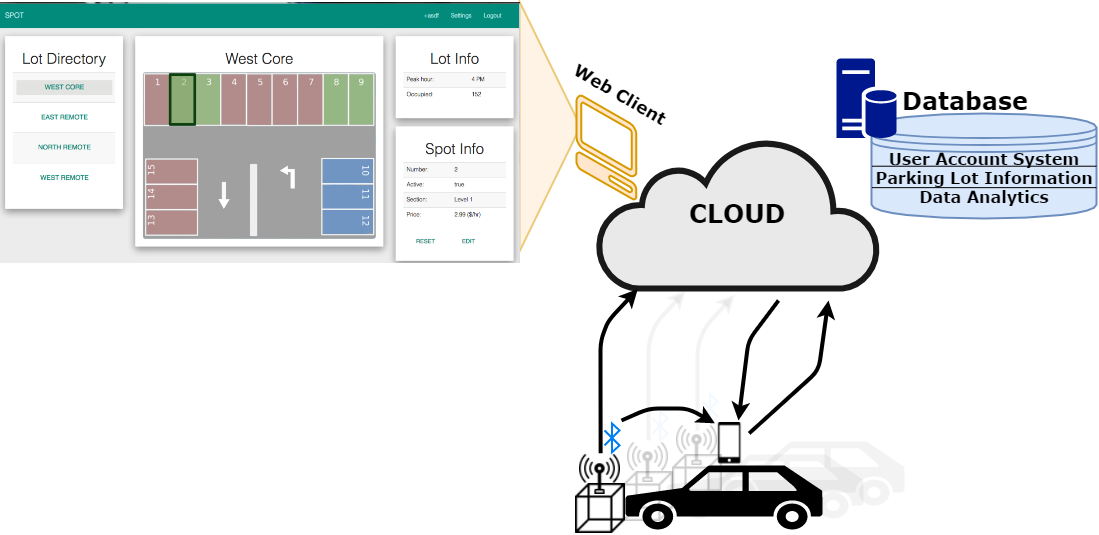
\includegraphics[width=0.85\textwidth]{pictures/SystemOverview.png}
\caption{System overview diagram showing communication paths between the cloud, sensor modules, website, and phone application.}
\end{figure}
%%%%%%%%%%%%%%%%%%%%%
For our implementation, we focus on if a car is about two feet in front, we will capture the license plate, run license plate recognition software, then simultaneously update the database with the current information and broadcast a Bluetooth beacon.
That exact same Bluetooth beacon that is broadcasting the uuid, was assigned by the Cloud.
Consequentially, it is picked up by the user’s phone that prompts a user sign-in/sign-up, payment option and a notification if they arrived at the specific stall. 
The Cloud works on providing the user and owner of the parking location an environment where both users can easily navigate and pursue the necessary actions they require. 
While hosting such services, the Cloud also performs its database duties by holding all information for every imaginable aspect: user account, individual sensor status, time of occupancy, structure/section pricing rates, etc.  
SPOT’s eventual goal is to provide a system that works far more efficiently for both drivers and managers of lots compared to today’s current parking system. 
%--------------------------------------------------------------
%   SECTION NAME
%--------------------------------------------------------------
\newpage
\section{Hardware \& Sensors}
% Here we can discuss the Hardware components of the raspberry pi and why we chose such a device (GPU, GPIO, Bluetooth, WiFi, etc.)
In the early stages of development for our system, we prioritized the ability for fast prototyping over power efficiency. 
Since we pursued overpowered functionality for image processing, easy programmable GPIO pins, and wireless communication via Bluetooth and WiFi, our decision for a single board computer Raspberry Pi Model 3 was perfect.
Raspberry Pi Model 3's have been commonly known as amazing tools for creating projects extremely fast with its System On Chip (SOC) with a multi-core processor, GPU, I/O peripherals, Ethernet port, USB host, and so much more.
Using these Raspberry Pi's for sensor modules, we easily produced multiple sensors for communication with the database. 

\subsection{Background Setup Process} %I Hate this title
For ease of mass production and automation for sensor modules on our developmental side, we created shell scripts specifically for setup.
A key aspect of modifying our sensors was allowing secure shell (SSH) connection through pipeline via internet.
To properly install this framework into our sensor modules is by using:

\vspace{0.5cm}
\begin{lstlisting}[language=bash]
sudo apt-get install sshpass
\end{lstlisting}
\vspace{0.5cm}

One main component for easy debugging was the ability for direct connection with each individual sensor module through WiFi addressing.
Using SSH allows us to easily modify or test each individual sensor based off of their unique identifier.

Another installation needed to operate the Raspberry Pi's properly for our functionality is the GPIO pins.
Our sole purpose for GPIO programming is for the proximity sensors.
\vspace{0.5cm}
\begin{lstlisting}[language=bash]
sudo apt-get install python-dev python-rpi.gpio
\end{lstlisting}
\vspace{0.5cm}

% With 40 GPIO pins for each sensor module is obviously overkill, but allows room for expansion with features
By installing these two specific packages, we can fully implement the python library for GPIO operation.

The same setup script includes creating a local log folder containing all the files for occupy status, time stamps, and uuid.
Creating these files locally allows us to individually control and track information for each individual sensor independent from connection to the database.

The last part of the script initializes boot-up daemons to automatically run once the sensor is powered on.
\begin{lstlisting}[language=bash]
sudo cp ~/scripts/setup/sensor\_nodes/bootup\_ping\_script.sh /etc/init.d/
sudo update-rc.d /etc/init.d/bootup\_ping\_script.sh defaults
\end{lstlisting}
These two lines solely edit the initialization files so when the device is powered, it runs our boot-up script.
Once these files are implemented into the daemons, the sensor is able to be completely automated.
\subsection{Sensor Automation}
%%%%%%%%%%%%%%%%%%%%%%
\begin{figure}[ht!]
\centering
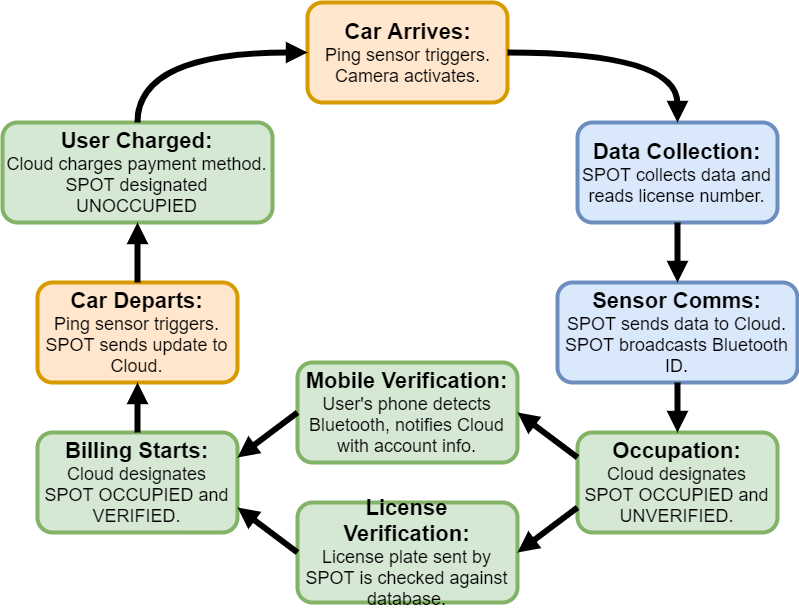
\includegraphics[width=0.7\textwidth]{pictures/EventFlowchart.png}
\caption{This demonstrates the flowchart that it continually repeating whenever a new car arrives at a SPOT.}
\end{figure}
%%%%%%%%%%%%%%%%%%%%%
For the convenience of administrative users, hardware operations are completely automated.
Using a Linux OS, we accomplished the automation through crontab. 
Crontab is a daemon that typically comes natively through Linux distributions. 
By editing the crontab file, we could schedule a single program to run periodically. 
However, we soon discovered this would not suffice because crontab had a minimum period of one minute and we needed to ping the spot at least every five seconds.
Periodically, we used a bash while loop to make a daemon that implements Linux calls like ‘sleep()’ to halt our program.
To send this process to the background we append ‘\&’ which commands a program to be thrown into the background. 
Altering these daemon background scripts allows our system to be initialized upon boot-up.
To avoid the program from throwing a signalling a close interrupt (SIGINT) error, our program is ran by ‘nohup’ which served to stop the program from throwing SIGINTS.
\begin{lstlisting}[language=bash]
nohup /pathto/program.sh \&
\end{lstlisting}

In our case we use:
\begin{lstlisting}[language=bash]
nohup  $\sim$/SPOT/scripts/setup/sensor\_nodes/background\_ping.sh \&
\end{lstlisting}

This was the specific file path and format for us to be able to run the background script.
In our file \textit{background\_ping.sh}, a series of scripts are called that automated the sensor module.
In the early stage of the script, we call python files that control GPIO peripherals for control over the proximity sensor.
After the python is executed for detecting if a car has approached the sensor module or not, a local status file is then written based from the results of the python. 
After the status is changed, we check to see if it is occupied or empty.
If the SPOT is occupied, we emit a red light and broadcast an eddystone beacon allowing the user to connect via our phone application. 
On the contrary, if the SPOT is vacant, a green light is emitted.
Once the status change is detected, the sensor uses a transfer script using a python function call to POST to the database with all the information needed for full functionality.

\subsection{Bluetooth Beacons}
%%%%%%%%%%%%%%%%%%%%%%
\begin{figure}[ht!]
\centering
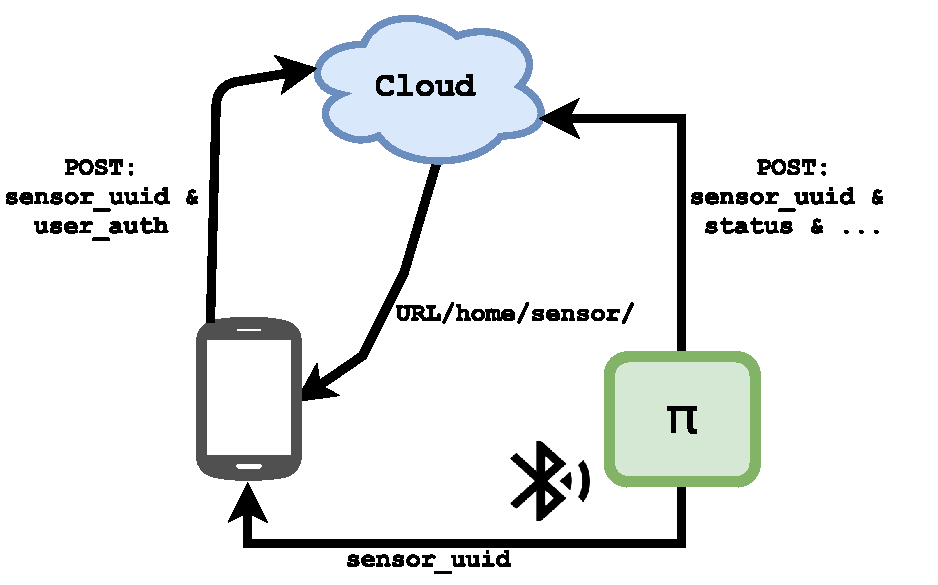
\includegraphics[width=0.85\textwidth]{pictures/BluetoothBeacon.pdf}
\caption{The process in which the user gets notified from the Bluetooth beacon, posts to the cloud their information, and gets redirected from the server.}
\end{figure}
%%%%%%%%%%%%%%%%%%%%%
Eddystone is a beacon format that can be used on both Android and iOS. 
Through the EddyStone Bluetooth Connection, we are able to format the payload in four different formats: UID, URL and TLM, EID. 
In the earlier stages of the project, we approached the broadcast as a simple URL using parameters to send specific information back and forth. 
This technique brings us a simple and direct way to link a URL with one or two parameters through Bluetooth. 
Unfortunately, this technique is extremely limited and the URL itself takes most of the bytes, while UID saves almost all the bytes for unique identification. 
The format each SPOT broadcasts is the UID format capable of broadcasting 20 bytes when activated.
With 20 bytes of being able to uniquely identify our sensor modules we have plenty of room for scalability. 
Using the phone application, we pick up the sensor's UID, tie it with the user account, then post to the cloud.

The UID payload has the following format:
\begin{center}
\begin{tabular}{ |c|c|c|c|c| } 
 \hline
 Frame Type & Tx Power & Namespace & Instance & Reserved For Future \\ 
 \hline
 1 byte & 1 byte & 10 bytes & 6 bytes & 2 bytes \\ 
 \hline
\end{tabular}
\end{center}
To set up the Raspberry Pi as a beacon we use this script:
\begin{lstlisting}[language=bash]
$\sim$/SPOT/scripts/setup/sensor\_nodes/eddystone\_test\_setup.sh
\end{lstlisting}
This script incorporates the HTTP GET and POST calls for generating unique uuids per sensor to alert the database specific information like which exact SPOT they have arrived at, and who exactly arrived. 
The eddystone broadcasts the sensor’s uuid for the phones to connect and redirect with.
Since Raspberry Pis have built-in Bluetooth capabilities we can simply run a command \textit{hcitool} that allows us to customize the information broadcasted with the proper url redirect and the uuid attach to the sensor notifying the server. \footnote{https://webgazer.org/update/tutorial/2016/03/16/raspberrypi-eddystone-url.html}

\begin{lstlisting}[language=bash]
hciconfig hci0 up
hciconfig hci0 leadv 3
hcitool -i hci0 cmd 0x08 0x0008 17 02 01 06 03 03 aa fe 0f 16 aa fe 10 00 02 77 65 62 67 61 7a 65 72 08 00 00 00 00 00 00 00 00
\end{lstlisting}

The the first sample of code enables on the Bluetooth capabilities of the Pi.
The next line allows us to broadcast a Bluetooth signal, by advertising a connection but not being able to fully connect.
This mean we allow the users to pick up the signal and read details from the advertisement, but prohibit users from connecting and altering the state of these Bluetooth connections.
When the server returns the successful notification of user connection, the user will be prompted a web page on their phone.

\subsection{Power Consumption  \& Analysis}
\begin{figure}[ht!]
\centering
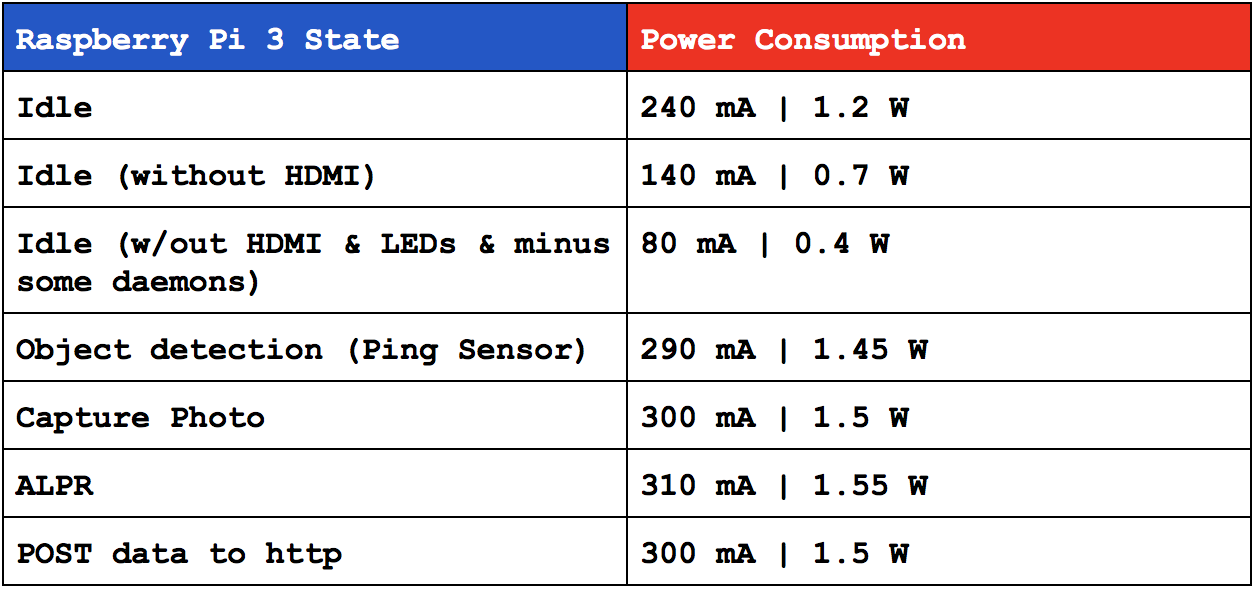
\includegraphics[width=0.9\textwidth]{pictures/Pipower.png}
\caption{This table shows the current power comsumption without the neopixel ring}
\end{figure}

As stated earlier in the document, power consumption was not the strong suit of this system. 
Given the table provided, we can immediately see the high current draws for idle states of the Raspberry Pi. 
When using high processing power with the image processing or communication to the database, we noticed a huge spike in energy consumption. 
When turning off the HDMI output port on the Pi, that took about 25 mA current draw off. 
By eliminating all the LEDs we brought our voltage down 5mA per LED. 
By disabling a few daemons on the Raspberry Pi  we got our current down by 100 mA or even more. 
We did not want to disable everything on the pi upon boot up. 
Overall we were able to limit the Raspberry Pi down to about 80 mA current draw which was about 0.4W.
In California, electricity averages around \$0.1534 kWh. 
Powering this sensor modules for an entire year for 24 hours a day would average you about \$0.53.

It was always in our knowledge to think of multiple directions we could optimize the energy consumption of each of our sensor modules.
Since SPOT is more of a system, we decided that energy consumption was by far the least of our worries and focus of the project.
In the future work discussion of this system document we will go into more detail about more viable solutions towards making our sensor modules optimal both with energy and functionality.
%%%%%%%%%%%%%%%%%%%%%%%%%
\subsection{Sensors}

\subsubsection{Proximity Sensing}
%%%%%%%%%%%%%%%%%%%%%%
\begin{figure}[ht!]
\centering
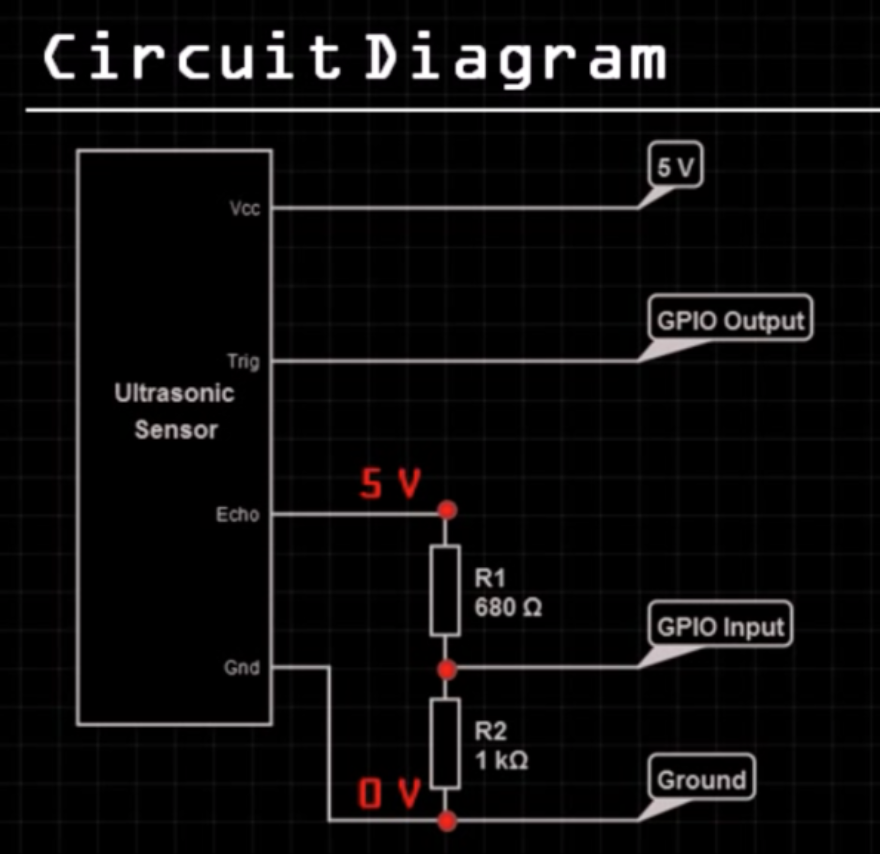
\includegraphics[width=0.5\textwidth]{pictures/ping_circuit.png}
\caption{This circuit shows our voltage drop across the echo to ground bringing the range from 0 to 5 volts down to around 0 to 3.3 volts into the GPIO input on our Raspberry Pi.}
\end{figure}
%%%%%%%%%%%%%%%%%%%%%
Our entire system and sensor module rely heavily on the sensors for proximity.
For our purposes, the ping sensor of our choice was the HC-SR04.
The data sheet can be found at from the link provided at the bottom. \footnote{https://cdn.sparkfun.com/datasheets/Sensors/Proximity/HCSR04.pdf}

This sensor is not always the best in terms of speed, but it can accurately give us distance in meters, feet, etc. 
This device is sequentially triggered causing the sensor to output sonic bursts that eventually return back to the device through the echo pulse output, hence the bit of delay causing the sensor to be a proximity tool. 
For our implementation we have the sensor connected through the GPIO pins on the Raspberry Pi through the circuit shown in Figure 4.
This voltage drop allows us to read precise measurements for the echo input into the Raspberry Pi. 
Since this ping sensor is extremely linear, round object detection does not always echo perfectly back.
The sensor is also on a time-based system, if the module does not hear back from the echo of the sonar pulse, it assumes there are no objects in front of it.
These two flaws are well known to us, but has not been proven to inhibit the ability of our proximity detection of a car pull into a SPOT.

Upon receiving the echo pulse output it returns a pulse width signal with the range in proportion.
This allows us to calculate the range through time intervals between sending a trigger signal and receiving an echo signal.

The reading conversion was quite simple:
\textit{
\begin{center}
    speed = $\frac{distance}{time}$
\end{center}
\begin{center}
         speed\ of\ sound = 340m/s = $\frac{2 \cdot distance}{time}$ 
\end{center}}
\begin{equation}
    distance = 170 m/s \cdot time
\end{equation}
%insert circuit design diagram

The python script we wrote functionally provides us with the ability to get accurate measurements for distances.

\begin{lstlisting}[language=Python]
while GPIO.input(ECHO)==0: # start timer 
  pulse_start = time.time()
while GPIO.input(ECHO)==1: # stop timer
  pulse_end = time.time()
pulse_duration = pulse_end - pulse_start
\end{lstlisting}

With the \textit{pulse\_duration}, we can easily use the time duration to calculate distance.
Upon initializing the Raspberry Pi for bumper detection in our file: \textit{bumper\_distance\_checker.py}, we set the GPIO pins for input and output.
Referring to the pinout from \ref{fig:rpi}, the pin we designated for \textit{GPIO.OUT} was 16 for the trigger output signal.

\begin{lstlisting}[language=Python]
GPIO.setup(TRIG,GPIO.OUT)
GPIO.setup(ECHO,GPIO.IN)
\end{lstlisting}
For the \textit{GPIO.IN} pin, we designated 18 for an input from the echo pulse response.
In the code, we set a short period of time, 1 milliseconds, allowing the ping sensor to settle then pulsed the trigger pin for a millisecond beginning the proximity process.

\begin{lstlisting}[language=Python]
GPIO.output(TRIG, True)
time.sleep(0.001)
GPIO.output(TRIG, False)
\end{lstlisting}

In the event if a person is simply crossing the sensor module, we trigger the sensor twice to make sure we get two very similar readings. 
If the error between the two proximity readings are above 10\%, we discard these results until the next period of measurements.
Once the two proximity measurements are accounted for and within the desired parking distance between the sensor module and the bumper, the sensor updates the local status file.
Once the Raspberry Pi is informed that there is an object in front via the status file, we continue to execute the rest of the automation script.

% Review this section
\subsubsection{License Plate Recognition}
Our system hopes to automate parking enforcement for our user. 
We leverage legally required licences plates, as a well instantiated form of visible ID, that can be used as a defense mechanism against unauthorized parking. Without camera-parsed license plate info, there’s no reliable way for our system to enforce appropriate parking. We’re currently using a well known algorithm OpenALPR to do all image processing for us right now. 
There's several dependencies to get OpenALPR running. OpenALPR directly depends on OpenCV and Tesseract, and Tesseract depends on Leptonica. All of these are image analysis frameworks required to get license plate recognition up and running.

Doing a pull from our github should give you all the setup script for openAlPR which install all dependencies. After everything should be ready to go! Depending on your drivers, you may need to update the camera driver to properly interface the OV5647 (RaspiCam). You can update to the appropriate driver using:

\vspace{0.5cm}
\begin{lstlisting}[language=bash]
$ sudo modprobe bcm2835-v4l2
\end{lstlisting}

With everything setup, you should be analyze a licencs plate using the following command:

\vspace{0.5cm}
\begin{lstlisting}[language=bash]
$ alpr check_myPlate.png 
\end{lstlisting}

This will return a list of license plate ID's and their associated probabilities. We use the most probable one.

\subsubsection{Status Light}
The status light is comprised of a Neopixel ring that is controlled by an Arduino Nano.
The Raspberry Pi controls the Arduino Nano through USB Serial communication. 
The necessary library can be easily installed by pressing \textit{Sketch \textgreater Include Library \textgreater Manage Libraries} and then:
\begin{verbatim}
#include <Adafruit_NeoPixel.h>
\end{verbatim}
The required setup on the Ardiuno files for serial communication requires:
\begin{lstlisting}[language=C]
Serial.begin(115200);
\end{lstlisting}
The Pi will send a 1 or a 0 if the ping sensor is triggered.
The Arduino Nano is programmed to only switch between the color green and red based on if the value from the Pi is 0 or 1. 
Upon connection the Ardiuno Nano is loaded with code that will iterate continuously.
If the serial is available for communication:
\begin{lstlisting}[language=C]
incomingByte = Serial.read() - '0';
if(incomingByte == 1) color(RED);
else if (incomingByte == 0) color(GREEN);
\end{lstlisting}
When a car is not occupying the SPOT, the Neopixel ring will default to green (0), which means not occupied.
When a car is in front of the SPOT, the Nexopixel ring will change to red (1), which will signify to the user that they are officially occupying the SPOT and billing will begin shortly. 
This UART connection is constantly running in the background so that the status light shown in \ref{fig:occupy} will change once the ping sensor triggers and notifies the cloud that there is a car.

\begin{figure}
\centering
\begin{subfigure}{.4\textwidth}
  \centering
  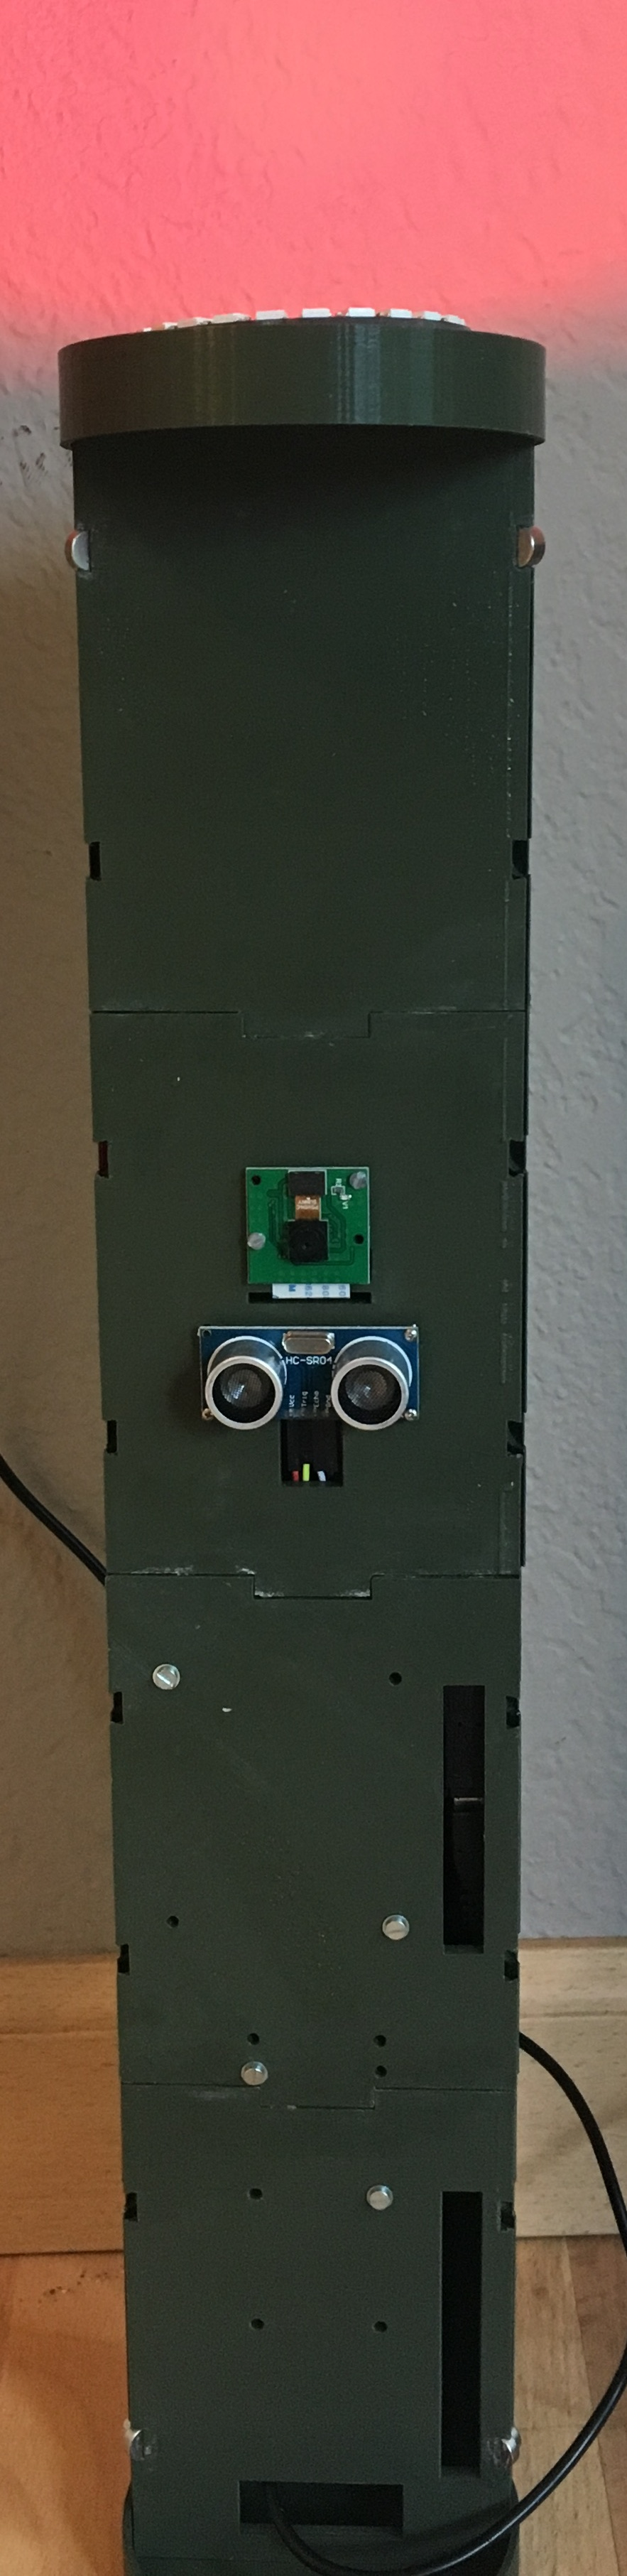
\includegraphics[width=.27\linewidth, height=8cm]{pictures/IMG_1664.JPG}
  \caption{SPOT with status: Occupied}
  \label{fig:3dprinted}
\end{subfigure}%
\hfill
\begin{subfigure}{.5\textwidth}
  \centering
  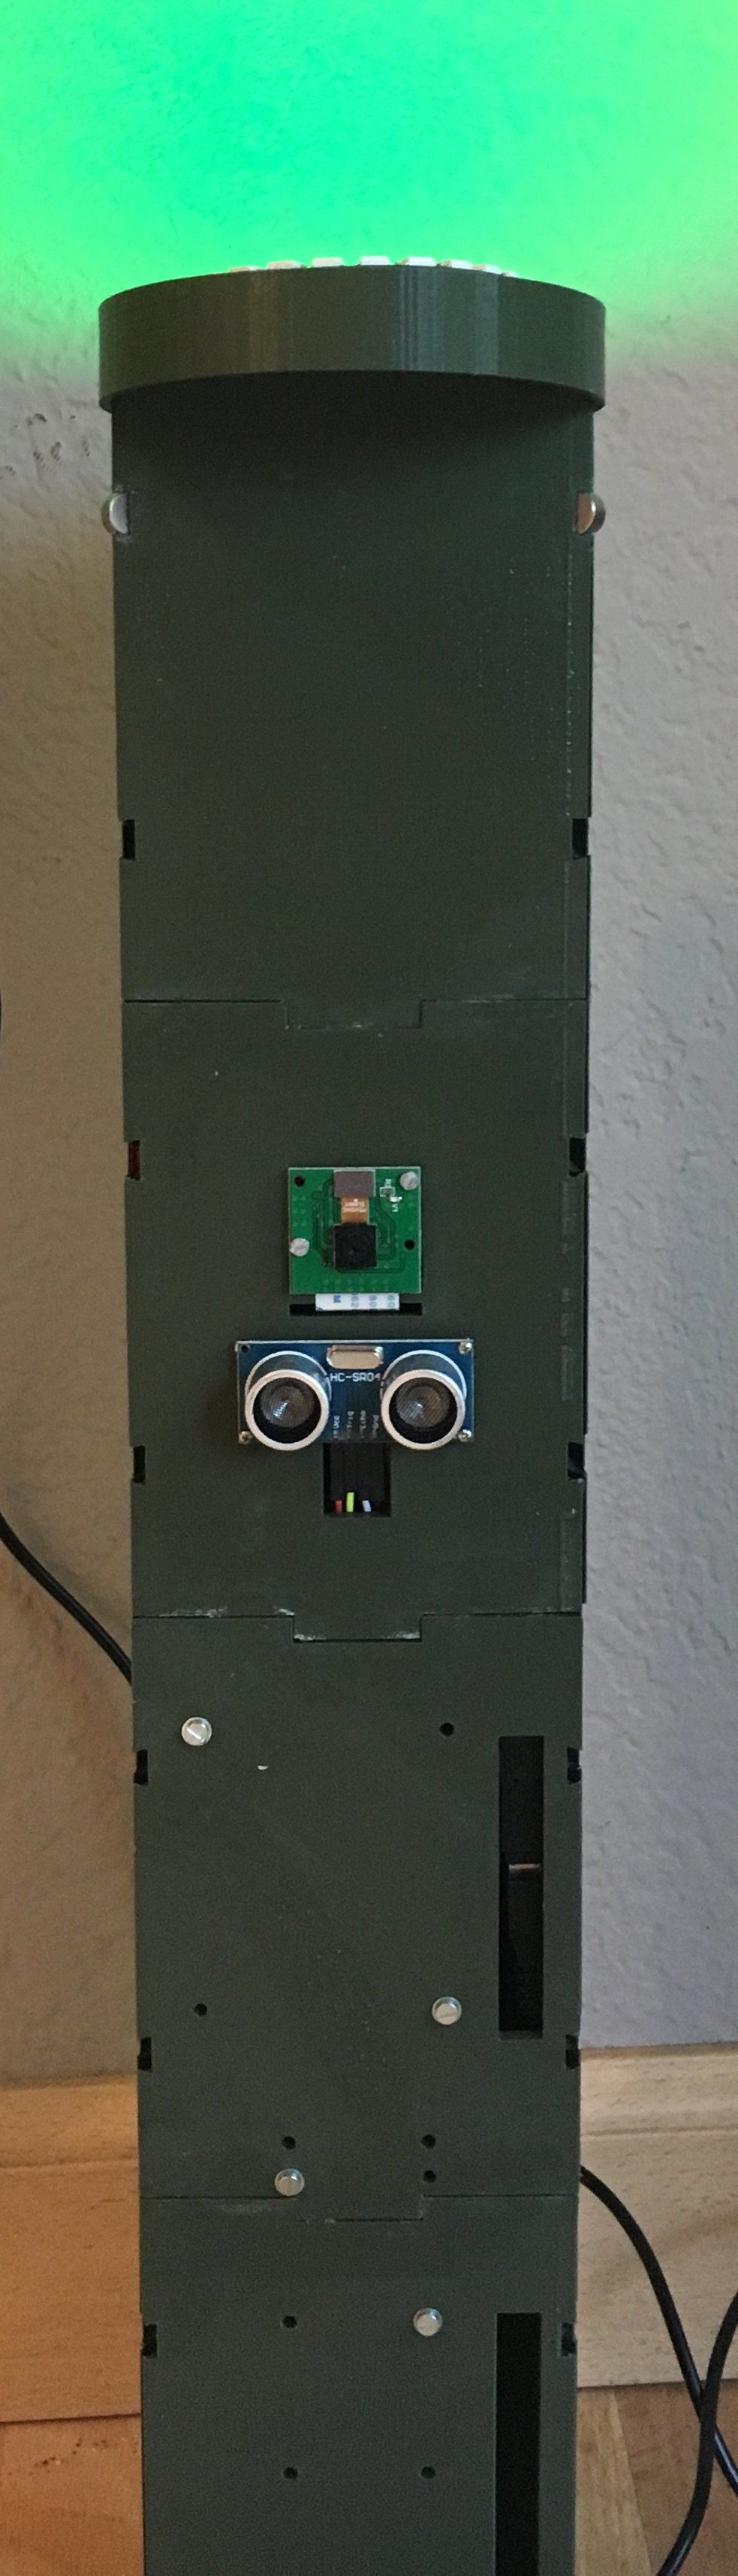
\includegraphics[width=.27\linewidth, height=8cm]{pictures/IMG_1668.JPG}
  \caption{SPOT with status: Unoccupied}
  \label{fig:acrylictube}
\end{subfigure}
\caption{Side By Side of Status Lights}
\label{fig:occupy}
\end{figure}

% \subsection{Future Implementations}%rephrase please, if you know a better one
%In here we can discuss other hardware & sensor options and briefly describe why we didn't use them or think these would be perfect from here on out
% Shouldn't we just be doing this in the future_work section?


%--------------------------------------------------------------
%   SECTION NAME
%--------------------------------------------------------------
\newpage
\section{Mechanical Design}
%We currently made two prototypes for our parking sensor box. The first iteration was too big and bulky. 
%To improve upon this, we made the section iteration way smaller.

%The idea behind our first design was to not reinvent the curb, we wanted a foolproof way to protect the sensor box while being far enough away to take a photo of the license plate, of the oncoming vehicle, when the ping sensor is triggered. 
%The first design has a self and is super spacious to hold all the components necessary.
%Ideally this design could latch onto an already existing curb or just sit as a standalone sensor that is behind the curb. 
%The section iteration  is essentially just thin and tall. The way we have it set up, the lcd screen, camera, ping sensor and pi will all be mounted vertically  on the back panel. 
%This way it'll save space so we don’t need such a wide box. With this new design, we can save some space and a more convenient size.  
%It has all the same functionality as the previous iteration, however now all the sensors and the raspberry pi are mounted vertically on the back panel of the sensor box. 
%This allows us to make a thinner box while still being able to house all the necessary sensors. 
%We can event make this customizable and add other sensors if we choose to. %wc

\begin{figure}
\centering
\begin{subfigure}{.4\textwidth}
  \centering
  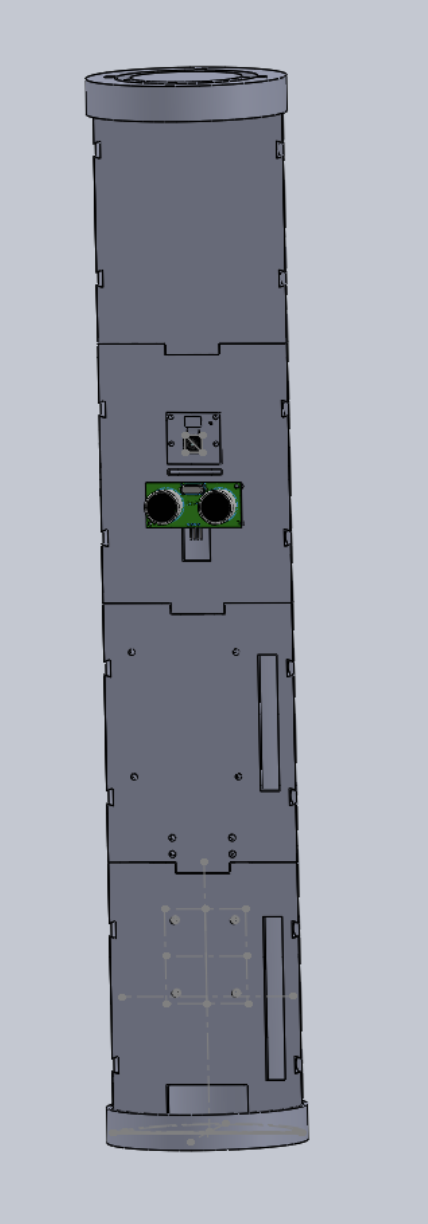
\includegraphics[width=.55\linewidth, height=8cm]{pictures/3Dprinted.png}
  \caption{CAD of The Sensor Unit: 3D printed parts assembled}
  \label{fig:CAD3dprinted}
\end{subfigure}%
\hfill
\begin{subfigure}{.4\textwidth}
  \centering
  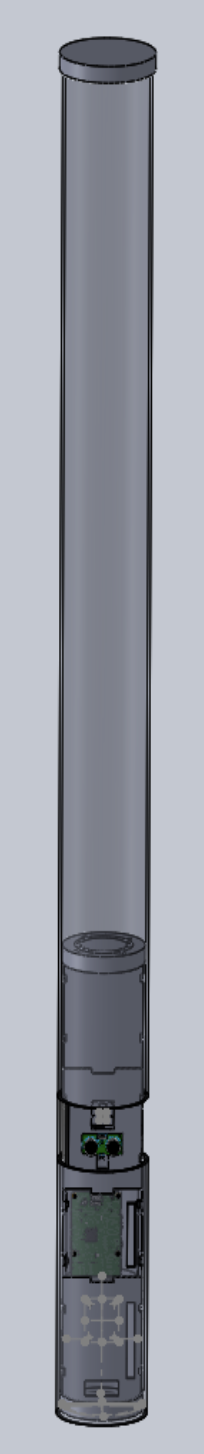
\includegraphics[width=.2\linewidth, height=8cm]{pictures/SensorTube.png}
  \caption{CAD of Sensor unit housed in a cylindrical acrylic tube}
  \label{fig:CADacrylictube}
\end{subfigure}
\caption{Our final mechanical design}
\label{fig:finalcad}
\end{figure} 
Our mechanical design prototype is comprised of 3D printed parts and an acrylic tube. 
We were limited by the factors that we wanted to create a low cost sensor housing prototype, that could be installed without having to alter a parking lot. 
Mostly due to the fact that if a parking lot has to be modified, it puts a parking lot out of commission for a period of time for construction and it is also costly to upgrade a parking lot or structure. 
It's also important to note that the mechanical design is not a major focus of our project, we just needed a method to gather data to send to the cloud. 

    We 3D printed parts most of the sensor housing system, which can all be found in our Github.\footnote{https://github.com/dfarley1/SPOT/tree/master/CAD}
There are 4 rectangular pieces that all tab and slot together. 
They can easily be glued together with tacky glue or epoxy. 
You need to put the pieces in the correct order, just so you can assembly it properly. 
We recommend taking all components to ACE hardware to get the correct sizing for each senor you would like to mount.
There are also magnets on the sides to allow for complete closure of of the 3D printed parts.
%%%%%%%%%%%%%%%%%%%%%
From top to bottom: this just a space holder, then the next panel holds both the ping and camera, following that the Raspberry  Pi is mounted, with another final bottom space holder.
% The order goes, the top piece is the top spacer then the piece that holds the sensors, then the piece that holds the raspberry pi and then then bottom spacer. 
The small lids (3.5 inches) go on either end and then you place the sensor box into the tube. 
To prepare the tube, you must cut it to the desired height and cut a window that is approximately 3 inches wide. 
This window must match up with the height of the of the 3D printed portions (once glued together).
You must also line the tube with wax paper in order to better capture the light from the pixel ring. 
This step allows for a better status indicator. 
Once assembled together it give us a sleek design of a semi circle that now fits into the acrylic tube.
Now place the 4 inch lids on either end of the tubes to help support the structure and provide a flat base. 
To hold the whole device, we obtained a 4 inch sprinkler head and the acrylic tube slides perfectly inside (after some sanding).

    For our final design, we opted for a cylindrical look to incorporate a sleek design.
Because the sensor housing device, is less than 2 feet tall, is quite short, most users would run it over easily. 
The addition of the acrylic tube was added so that users would be able to see the status of the SPOT from the car and prevent the user from running it over. 
With this iteration it was important to maximize the space of the 3D printer so each piece is approximately 4.5 to 5 inches tall each. 
Combined all together with some glue, the 3D printed portion of the mechanical design holds the camera and ping sensor at a proper height of 10-11 inches off the ground.
This is so that our prototype can detect whether or not a car is right in front of it or not. 
The Raspberry Pi is hidden inside the semi circle so that all the wires are enclosed and it is neat and tidy from an outside point of view. 
We also added some magnets to help enclose the entire module. 
This way we can open and close the module with ease whenever we need to do some testing. 
The 3D printed parts were very sturdy, however it took a long time to print one set in order to assemble the whole system.

\begin{figure}
\centering
\begin{subfigure}{.4\textwidth}
  \centering
  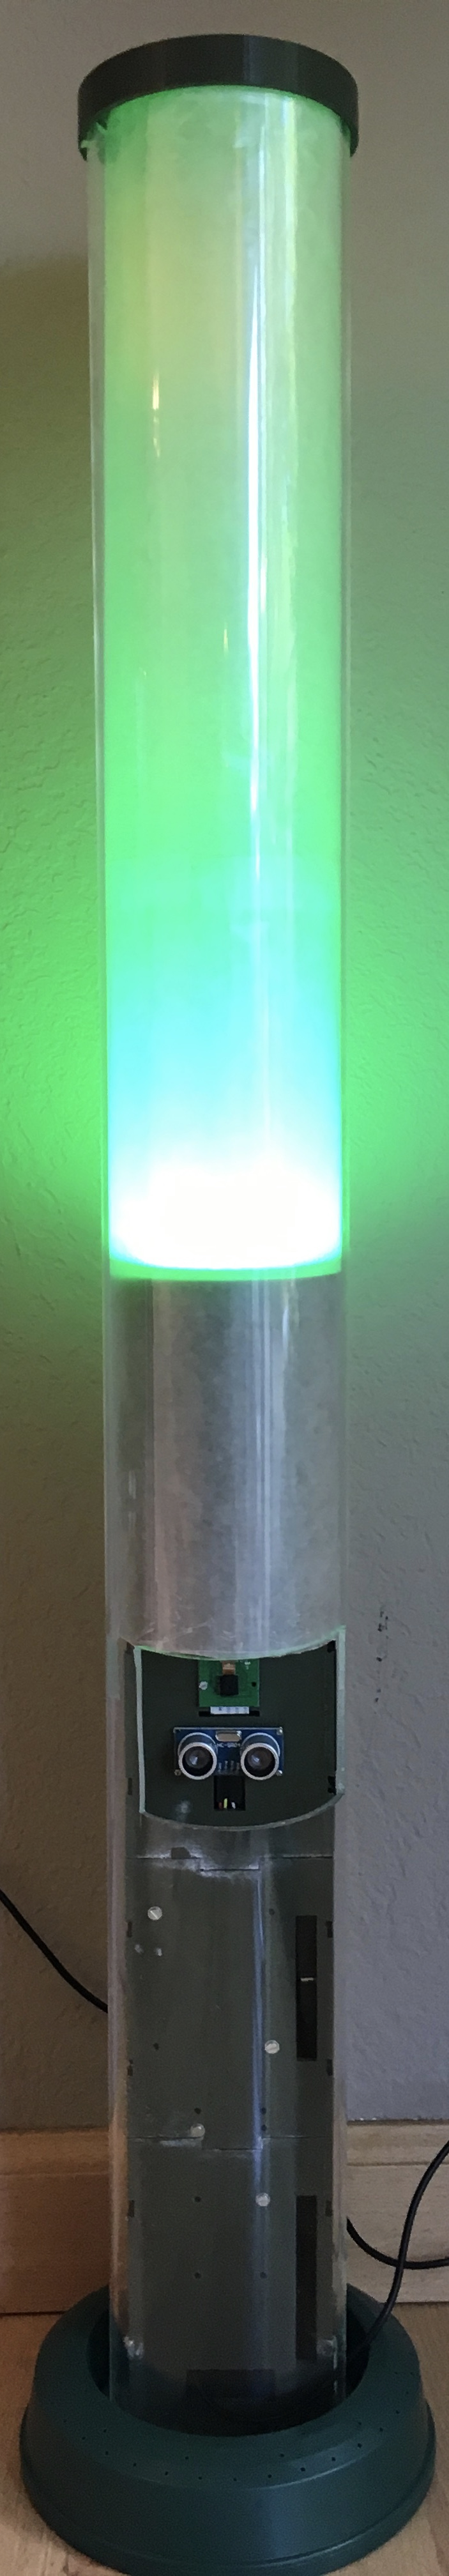
\includegraphics[width=.25\linewidth,height=9cm]{pictures/fullsizeoutput_14d.jpeg}
  \caption{Physical Prototype: SPOT with status: Occupied}
  \label{fig:3dprintedassembly}
\end{subfigure}%
\hfill
\begin{subfigure}{.4\textwidth}
  \centering
  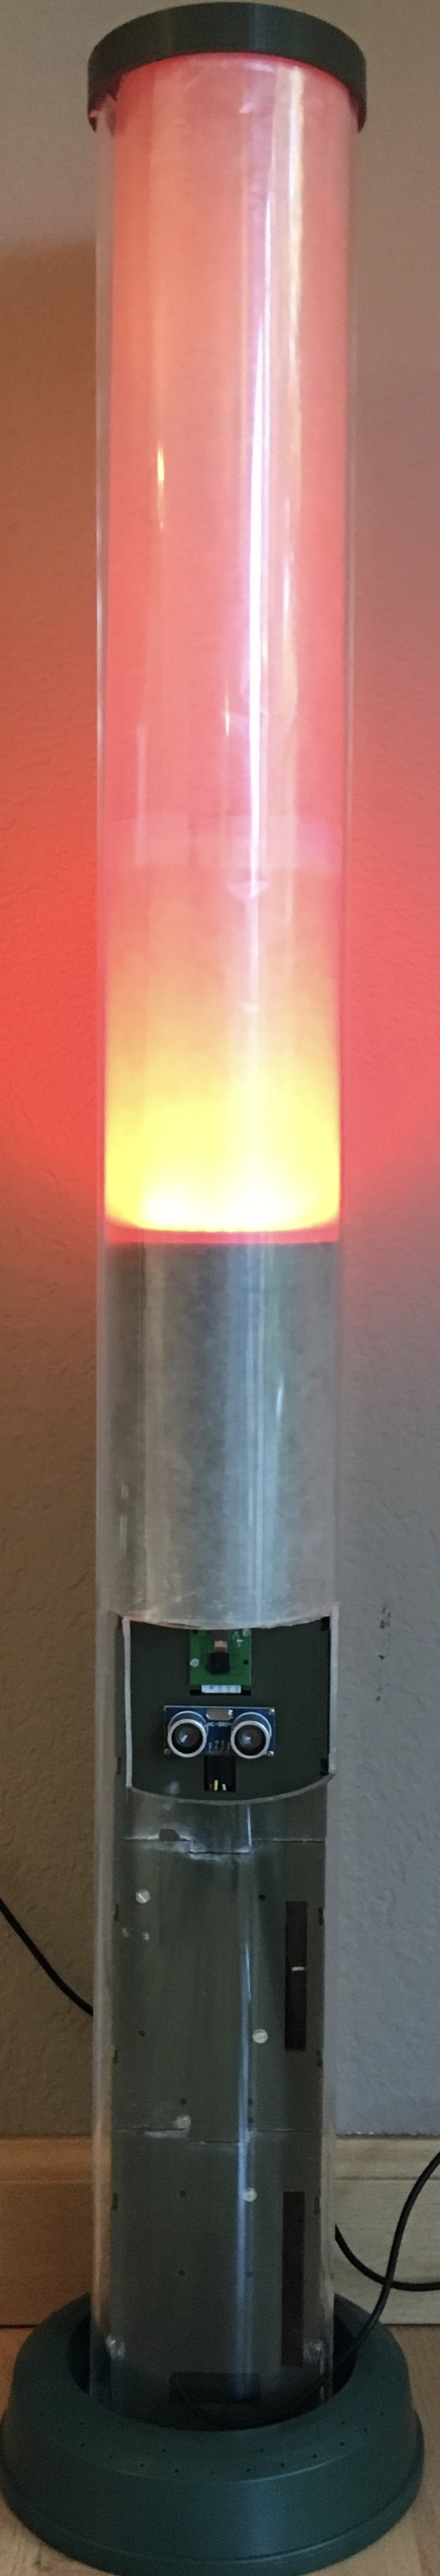
\includegraphics[width=.25\linewidth,height=9cm]{pictures/fullsizeoutput_14f.jpeg}
  \caption{Physical Prototype: SPOT with status: Unoccupied}
  \label{fig:acrylictubefullassembly}
\end{subfigure}
\caption{Physical Prototype: Side By Side of Status Lights with Acrylic Tube}
\label{fig:finalassembly}
\end{figure}


%--------------------------------------------------------------
%   SECTION NAME
%--------------------------------------------------------------
\newpage
\section{Cloud Server}
% This will be the quick overview/background to Cloud

%How we get the data (django and REST APIs), what we do with the data (database, analytics), and how we present it (website, phone)

We developed a web server application to serve as the primary coordinator of the system.
The server has several key responsibilities: exchanging information with SPOT sensors and user's smart phones, managing our database, and implementing a user account and billing system.
It must also serve a public-facing website for drivers and lot managers, perform real-time and historical data analytics, and provide endpoints to access the calculated data.

In order achieve these goals we relied primarily on the Django web framework and Django REST Framework library running on a Google App Engine instance.
Django is a web and REST framework written in Python which provides the backbone of our system including API endpoint generation for mobile, web, and sensors, user account management, data analytics, and real-time SPOT tracking.
The Google App Engine platform allows us to quickly and easily deploy web server code that is accessible from anywhere via an Internet connection with near-limitless scalability, automatic load balancing, and near 100\% up-time.

%%%%%%%%%%%%%%%%%%%%%%%%%%
\subsection{Setup Tutorial}
Our primary guide for setting up the development environment came from Google themselves.\footnote{https://cloud.google.com/python/django/appengine}
This tutorial walks through setting up the project instance on GCloud and commands needed to deploy our code to the server.
It also outlines the packages and libraries needed to run the server locally.
Additionally Google provides an SQL proxy application which allows your locally-running server to use the GCloud MySQL instance, which allowed us to share one database between team members and collaborate using common data.

We also utilized Visual Studio Code\footnote{https://code.visualstudio.com/}, a new IDE by Microsoft aimed at web application development.  On top of all the usual features like code completion and file management it also provides debugging and breakpoint services for both our Python and JavaScript code.
Using VSCode was incredibly helpful for development and did not require any additional configuration, it has predefined setting profiles for Django built in.

%%%%%%%%%%%%%%%%%%%%%%%%%%
\subsection{Back-end}

\subsubsection{Django}
Django is a web framework platform which follows the Model-View-Template pattern.
We used version 1.10.5, the latest stable release available that the Google App Engine officially supported.\footnote{https://docs.djangoproject.com/en/1.10/}
Throughout the development process there were not any major changes between versions that warranted upgrading.
\begin{itemize}

\item A Model refers to the database abstraction layer Django provides which allows developers to interact with a database in a purely Pythonic manner using dictionary like classes, there is no need to manually write SQL queries.
\item A View is the Python function which is called when an HTTP request is sent to the server.
Within this view parameters are parsed and analyzed, database exchanges are made, logic is performed, and output is determined.  The URL being requested can be parsed in order to determine which view should be called on the request.
\item A Template is used to deliver HTTP content as a response to the sender. 
A template contains both HTML markup and Python code. 
When the template is rendered by the View, the Python code is evaluated and a final HTML file is replied to the sender.
\end{itemize}
  

When a client makes an HTTP request to the server it can be in one of two forms: a GET or a POST message.
A GET message is used to request certain information from the server and does not alter any information on the server's side.
The GET message can specify parameters to narrow down the scope of data being requested.
For example a web client might submit a GET request for a specific user's parking status and use that user's email address as a parameter to the request.
A POST message is used to submit new or updated information to the server.
A POST message can also specify parameters to narrow the scope of data that it is updating.
For example, SPOT sensors submit a new POST request with their UUID as a parameter whenever they detect a car arriving or leaving.

Using Django allowed us to quickly and easily deploy new endpoints for the sensors, phones, and website to interact with as well as implement complex relational models and analytics.

%TODO overview of the apps we used


\subsubsection{Django REST Framework} %How JSON works and provides an easy way to transmit arbitrary data structures
On top of the standard Django framework we deployed the Django Representational State Transfer Framework (DRF) version 3.5.4 library to facilitate arbitrary client-server data exchanges in a programmatic format when the data is not slated for immediate display to the end user.\footnote{http://www.django-rest-framework.org/}
For example, SPOT sensor boxes need to send data to our server when they detect changes in the environment but displaying this content is not necessary.
Instead data is sent in JavaScript Object Notation (JSON) format allowing us to exchange dictionary objects over HTTP.

DRF provides default and customize-able serializers and deserializers to convert Python dictionaries into JSON objects and back for both normal classes and those based on our Django database models, allowing us to quickly pull data from the database and send it to the client for our front-end to work with.


%%%%%%%%%%%%%%%%%%%%%%%%%%
\subsection{Data Collection}
At the core of SPOT is the ability for our server to capture and track the state of numerous sensors and deliver data about the sensor network to various client interfaces.
In order for clients (SPOTs, web interface, or phones) to send or receive data with the server we must define endpoints with which they can interact.  
From the client's point of view these endpoints look almost like function calls; parameters can be attached to the request which is sent to the server for processing and a response is returned.

SPOT's API defines a number of top-level categories which are defined in \verb|django/mysite/urls.py|:
\begin{lstlisting}[language=Python]
urlpatterns = [
  #templates
  url(r'^sensor/', include('sensor.urls')),
  url(r'^monitor/', include('monitor.urls')),
  url(r'^user/', include('user.urls')),
  #api
  url(r'^api/v1/auth/', include('authentication.api_urls')),
  url(r'^api/v1/monitor/', include('monitor.api_urls')),
  url(r'^api/v1/user/', include('user.api_urls')),
]
\end{lstlisting}

Each entry in this array specifies a URL string to match and which Django app it should forward to.  For example, URLs beginning with "\verb|sensor/|" will be forwarded to \verb|sensor/urls.py| for further routing.
The two primary resources for capturing system-state data are from sensors and user smart phone applications.

\subsubsection{Sensor Page: /sensor/}
Methods for sensors to establish themselves with the server, POST updates, and GET updated metadata about themselves from the server.

Note that code for this section was written before we implemented DRF and JSON data exchanges.
Everything is done in plaintext with no serialization; this should NOT be followed as an example.
\begin{lstlisting}[language=Python]
    urlpatterns = [
        url(r'getUUID/', getUUID.getUUID, name='getUUID'),
        url(r'^', sensor.sensor_main, name='sensor'),
    ]
\end{lstlisting}

\begin{itemize}
  \item \verb|getUUID|: Used by sensors to "register" themselves with the server.
  The server will generate a new UUID and blank database entry for the sensor and return the UUID to the sender.
  This process creates a new logical SPOT so it should only be done when a new sensor is installed.
  \item \verb|^|: This regex pattern matches anything and is the default route taken when no other patterns are matched.
  The primary interface for sensors to send and receive data with the server.
  \begin{itemize}
    \item A GET request to this URL must contain a valid UUID (obtained by a GET request to \verb|sensor/getUUID|) and returns a plaintext representation of the associated SPOT's database entry.
    \item A POST request to this URL must contain the following a valid UUID as a parameter as well as the following POST headers:
    \begin{enumerate}
        \item \verb|occ_status|: The new occupation status of the sensor: nominally "1" for occupied, "0" for unoccupied.
        \item \verb|occ_since|: A UTC timestamp specifying the time since occupantion status last changed.
        \item \verb|occ_license|: A string either containing the occupant's license plate or the empty string.
    \end{enumerate}
    The server retrieves the relevant SPOT entry from the database and updates the model with the new data passed from the sensor.
    Additionally if a change in state is detected (occupied to unoccupied or vice versa) then the logging system is triggered and updated as described below.
  \end{itemize}
\end{itemize}

\subsubsection{Phones}
As far as system data collection is concerned, the phones provide one event worth collecting: the detection of a Bluetooth beacon within proximity of the user.
This signifies that a nearby sensor has detected a car and began a Bluetooth broadcast.
After obtaining a login credential the phone can make a POST request to \verb|/api/v1/auth/occupy/| with detected sensor UUID.

Note that unlike the sensor API, this request uses the DRF allowing data to be transmitted via JSON.
Using this scheme is more appropriate when the data exchange does not rely on presenting the client with formatted HTML content and will be used throughout the rest of the project including most functionality developed for the front-end monitoring and website.

This request is routed through \verb|authentication/api_urls.py|.
\begin{lstlisting}[language=Python]
urlpatterns = [
  url(r'^login/$', LoginView.as_view(), name='login'),
  url(r'^logout/$', LogoutView.as_view(), name='logout'),
  url(r'^occupy/$', OccupyView.as_view(), name='occupy'),
]
\end{lstlisting}
Which specifies that the request should be handled by the \verb|OccupyView| class in the \verb|authentication/views.py| file.

DRF views are defined as classes with a function for each HTTP method which can be received by it.
\begin{lstlisting}[language=Python]
class OccupyView(views.APIView):
  permission_classes = (permissions.IsAuthenticated,)
  def post(self, request, format=None):
    data = json.loads(request.body)
    ...
\end{lstlisting}
\verb|permission_classes| specifies that all methods in the OccupyView require that the sending client is successfully logged in.
Authentication sessions are handled automatically by Django and stored client side in cookies.

The \verb|post| method, as the name suggests, handles POST requests sent to the URL.
Within this function \verb|data| contains the deserialized arguments sent by the client, including the detected beacon's UUID.
This UUID is used to retrieve the relevant SPOT Data database entry which is updated such that the SPOT is \textbf{occupied and verified}.
Additionally, the most recent Event Log entry is updated to include the user which is occupying the SPOT so that the system knows who to charge when they depart.

With input from the sensor modules and smart phones the SPOT system is receiving enough information to track who is parking where and for how long.
The next step is to organize, store, and analyze all of the collected data.

%%%%%%%%%%%%%%%%%%%%%%%%%%
\subsection{Models Overview}
Django provides a database abstraction layer which they call Models, or Python interface for database tables stored in a MySQL database on the Google Cloud.
A Model class defines the database table and its attributes while the member variables of that class specify the table columns and their datatypes.
An instance of the Model class represents a row or entry in the database table.
Models can be queried and sorted based on their fields to obtain an array of entries without any SQL syntax or type conversions; everything is handled by the DAL and presented as Python dictionaries.

\begin{figure}[ht!]
\centering
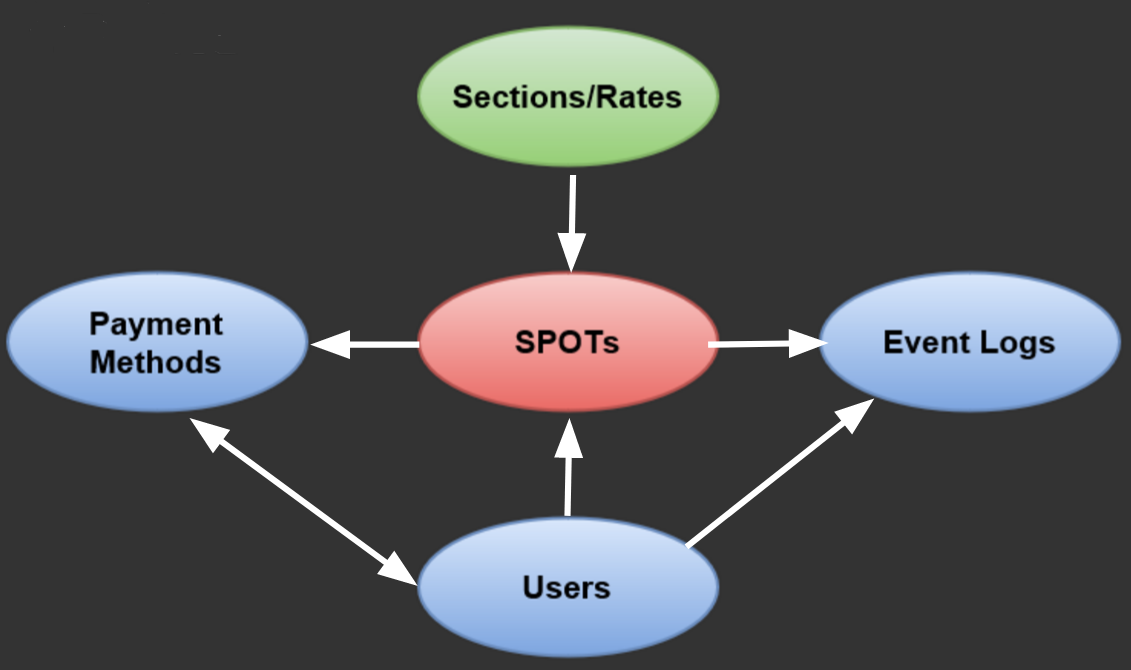
\includegraphics[width=0.85\textwidth]{pictures/models.png}
\caption{Relationships between database models.}
\end{figure}

In order to provide the basic functionality of knowing who parks where at what times, we need to keep track of two things: the SPOTs and the users.  
In addition to that we need an interface that lets us store pricing rate information, parking permit overrides, and historical logging for analytics.

\paragraph{SPOTs}
are the primary source of data in the system and maintain the "live" status of all sensors as well as some editable metadata about the SPOT.
\begin{lstlisting}[language=Python]
class spot_data(models.Model):
  uuid = models.UUIDField("UUID", 
      primary_key=True, unique=True)
  #"static" metadata about spot
  section = models.ForeignKey(sections, null=True)
  number = models.IntegerField("Spot Number")
  #"variable" current status
  last_update = models.DateTimeField("Last Update", 
      auto_now=True)
  occ_status = models.SmallIntegerField("Occupied Status", 
      default=0)
  occ_since = models.DateTimeField("Occupied Since")
  occ_license = models.CharField("Occupant License", 
      max_length=20)
  occupant = models.ForeignKey(Account, null=True)
class sections(models.Model):
  name = models.CharField("Section", max_length=100)
  structure = models.ForeignKey(structures, null=True)
  rates = models.TextField("Rates Array", 
      default=rates_default)
class structures(models.Model):
  name = models.CharField("Structure", max_length=100)
\end{lstlisting}
SPOTs have a UUID as a primary key so that each SPOT is easily identify-able and removing entries from the database is still extremely unlikely to produce duplicate identifiers.
The UUID is also 16 bytes, perfectly matching the Bluetooth beacon's UID size.  

SPOTs also contain some "static" geographic information about the SPOT such as a number, section, and lot.
These additional models are relatively minor themselves but allow each SPOT to be located and filtered based on its physical position.
SPOTs reference a Section that they belong in, which can be "level 1", "row A", etc.
Sections reference a Lot that they are part of, such as "West Core" or "Lot 151".

Lastly is the current live data about the SPOT: whether or not it's occupied and how long it's been in that state, who's parked there (if verification has occured) and any detected license plates.

\paragraph{User Accounts}
are necessary for drivers to register with the system so that SPOT knows who is parking where.
Luckily Django has a built-in interface for this which already provides login session management, registration, authentication, secure password storage, and other basic user account services.
In our current implementation we've only added a reference to payment methods that a user has purchased or authorized but future development will include being able to tie license plates and SPOT reservations to the user.
Currently there is not much we are using the User model for aside from all of the default functionality provided by Django; users are instead referenced by the other models and used to authenticate a driver.

\paragraph{Payment Methods}
are a list of permits and ways to be charged for parking.
\begin{lstlisting}[language=Python]
class payment_method(models.Model):
  name = models.CharField("Payment Method Name", 
      max_length=100)
  purchase_price = models.FloatField("Purchase Price", 
      default = 0.0)
  rate_modifier = models.FloatField("Rate Modifier", 
      default = 1.0)
\end{lstlisting}
Payment Methods can be thought of as an abstract class which can be extended to include credit cards, prepaid cards, old school tickets, or lot-specific parking permits as used by UCSC.
At the current stage of development they are almost a placeholder, only containing a purchase price and a "rate modifier".
This modifier is a basic percentage multiplier that is applied to the payment accrued while parking.

\paragraph{Event Logs}
are used to store the history of events that occur in the SPOT system.
\begin{lstlisting}[language=Python]
class event_log(models.Model):
  start = models.DateTimeField("Arrival", null=True)
  end = models.DateTimeField("Departure", null=True)
  total_paid = models.FloatField("Total charge", default=0)
  payment_method = models.ForeignKey(payment_method, 
      null=True)
  spot = models.ForeignKey(spot_data, null=True)
  user = models.ForeignKey(Account, null=True)
\end{lstlisting}
Each entry in the log is built to catalog everything about a driver's park in a SPOT.
When a SPOT detects an arrival a log entry is created with the SPOT being occupied and the time occupation began.
When verification occurs (either through license plate or Bluetooth) the log entry is updated to include the user account who was verified.
When a SPOT detects a departure the log entry updated with the time of departure, total amount paid, and payment used.

This catalog of events keeps the entire history of SPOTs available for future use.  The list of events can be filtered by a specific user account to provide a timeline or payment history.
It can also be filtered by SPOT, section, or lot for managers to calculate various usage analytics and display information on the web page.

\subsection{Payments}
SPOT allows lot managers to define hours of operation and parking rates in 15 minute increments across all seven days of the week.
This information is stored in a two-dimensional 7x96 float array where each value represents the hourly rate for that 15 minute interval.
Array indices and 24 hour times (00:00 - 23:59) can be determined with the following formulas:
\begin{equation}
    index = hour * 4 + \left \lfloor{minute / 15}\right \rfloor
\end{equation}
\begin{equation}
    hour = \left \lfloor{index / 4}\right \rfloor
\end{equation}
\begin{equation}
    minute = (index \% 4) * 15
\end{equation}
Index [0,0] represents Sunday from 00:00 to 00:15; [0,1] represents Sunday 00:15-00:30; [3,81] represents Wednesday 20:15-20:30; and so on.
Note that negative numbers are used to represent that the SPOT is unavailable att hat time.

Our current implementation calculates the total payment by building a rate mask of floats where each value is the percentage of the 15 minute interval that the SPOT was occupied.
That mask is then applied to the rate table for the SPOT's section, yielding an array whose values represent the amount owed for each 15 minute interval.
Summing all values in this array gives us the total amount owed, which is then multiplied by the rate modifier in the user's preferred payment method.

Future plans include redesigning this algorithm to improve reliability over multi-day parking and reduce overhead by instead walking through the time delta a SPOT was occupied and checking each applicable index in the array rather than building masks.

\subsection{Queries and Analytics}
Django's model interface allows database tables to be queried based on various field values, much like SQL.
For instance, all parking events for a user named "Daniel" can be retrieved and sorted by start time with the following code
\begin{lstlisting}[language=Python]
#get the user account for "Daniel"
Daniel_acc = Account.objects.filter(first_name='Daniel')[0]
#get the log entries associated with this account
Daniel_hist = event_log.objects.filter(user=Daniel_acc)
#sort them in decreasing order by the "start" field value
Daniel_sorted = Daniel_hist.order_by('-start')
\end{lstlisting}
Obtaining all of the SPOTs located on Level 1 of West Core is equally as simple:
\begin{lstlisting}[language=Python]
#get the lot named "West Core"
West_Core = lots.objects.filter(name='West Core')[0]
#get the "Level 1" section of West Core
WC_L1 = sections.objects.filter(lot=West_Core)[0]
#get the SPOTs in this section
WC_L1_SPOTs = spot_data.objects.filter(section=WC_L1)

#get SPOT 17, Level 1, West Core
WC_L1_17 = WC_L1_SPOTs.filter(number=17)[0]
\end{lstlisting}

Using Django's model interface allows us to perform complex database queries quickly and easily, allowing us to perform powerful analytics across multiple database tables.

%%%%%%%%%%%%%%%%%%%%%%%%%%
\newpage
\subsection{Front-end}
\subsubsection{Using Angular with Django}
Since we used Django Framework to to run our server, extra precautions were needed in order to avoid collisions with AngularJS syntax.
For example, to :
\vspace{0.5cm}
\begin{lstlisting}[language=html]

.
<p>{{ ang.binded_variable }}<\p>
.

\end{lstlisting}
\vspace{0.5cm}

Angular and Django are capable of binding data to HTML clientside and serverside, respectively.
Syntax collision occurs with angular bindings if they aren't wrapped in the code shown above.
This is because they both share data binding sytax of '{{ang.binded\_data}}'.
Pulling our github repository should set you up with the right structure.

\vspace{0.5cm}
\begin{figure}
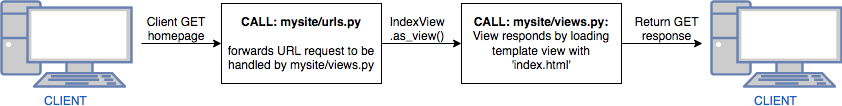
\includegraphics[width=1\textwidth]{pictures/Client_getIndex.png}
\caption{Sequence after a client requests the home page from our cloud server.}
\end{figure}

Next, let's load the home page.
Figure 10 shows a how the cloud server responds to a home page request.
Note how the Django View, different than ng-view, loads index.html into its response.
The django view gets handed HTTP requests and can deal with them as it wants.


\newpage
\subsubsection{Dynamic loading}
Responding with new HTML implies that the client should re-render, or refresh, their page.
To avoid unnecessary refreshes, we transferred new data through JSON files between server to client.
In this manner, we could communicate the addition of, for example, a new parking lot and have client-side AngularJS update the webpage seamlessly.
Instead of having to communicate new views via html, the server now encodes our data as JSON and Client-Side AngularJS decodes the json and updates the html view live.
This in an upcoming practice referred to as SPA (Single Page Application)

\vspace{0.5cm}
\begin{lstlisting}[language=html]
<div class="container-fluid">
		<div class="row">
			<div class="col-xs-12 ng-view"></div>
		</div
</div>
\end{lstlisting}
\vspace{0.5cm}

Angular allows directives to be integrated directly into HTML.
In this case, we use an ng-view element to dictate a dynamic HTML box in the DOM, that is the same size as the div it describes.
This becomes our dynamic environment wherein our AngularJS can dynamically update our home page HTML without re-rendering.
This includes having AngularJS dynamically inject entire HTML pages.

\begin{figure}
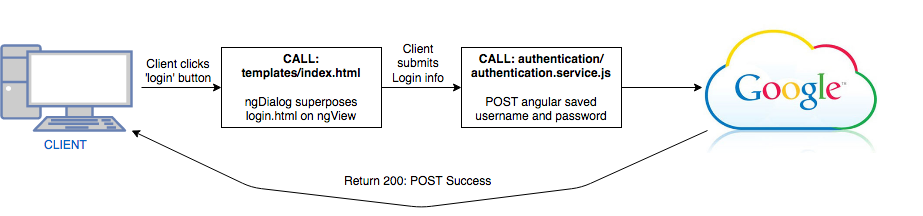
\includegraphics[width=1\textwidth]{pictures/Client_angRouting(2).png}
\caption{Sequence after a client requests the home page from our cloud server.}
\end{figure}

\newpage
\subsection{Website}
\subsubsection{Monitor}
\begin{figure}[htb]
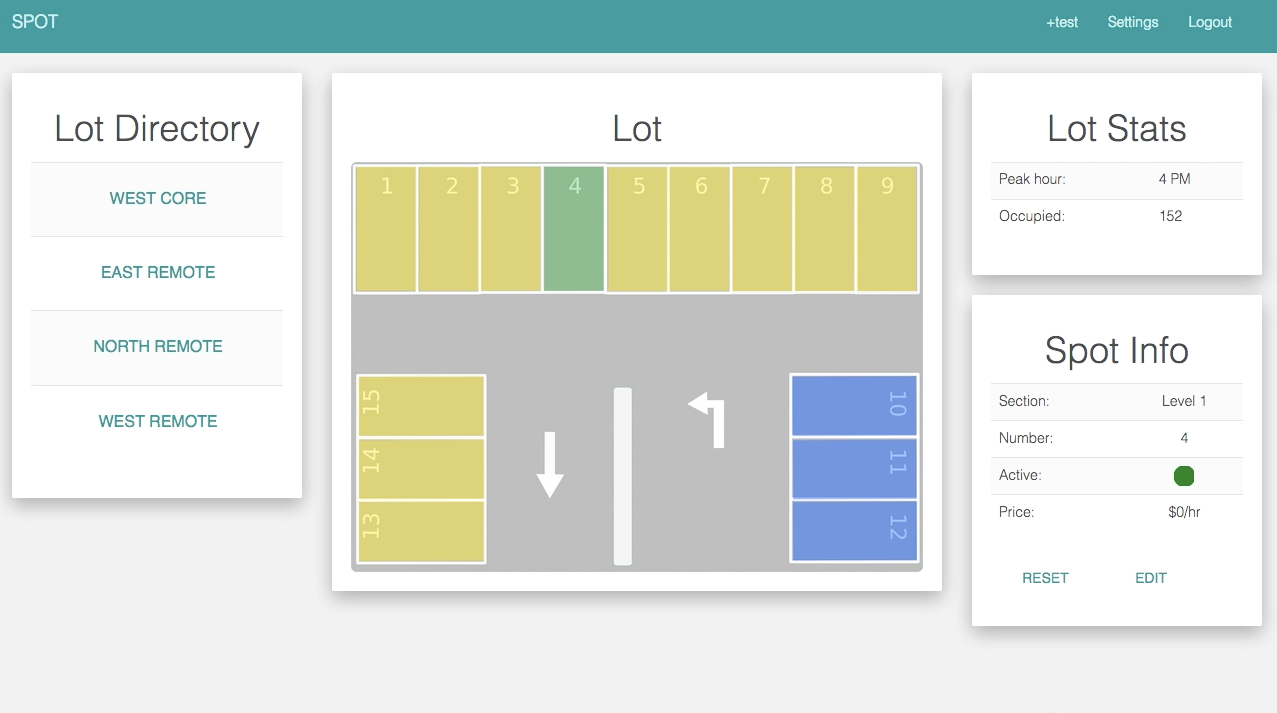
\includegraphics[width=1\textwidth]{pictures/MonitorScreen.png}
\caption{Screen shot of the finished monitor page.}
\end{figure}

After downloading a Django template project, you should find that there's a particular directory structure.
Note that django has a modular manner of splitting up large/related tasks into 'apps'.
For instance, we had an app 'monitor' which housed all the django python and html templates that related to our monitor page.
There are two main ways of returning a page. One can use Django URL routing (See django/monitor/urls.py) or by using the using Angular routers hooked with Django (See django/static/javascripts/sdpspot.routes.js).
The former can only modify HTML before sending it off to the client, while the latter can modify HTML after being received by the client.
Using angular routing, we developed a Web API that allowed us to SPA-update the user's page with info from our database:


\newpage
\begin{table}[!htb]
\renewcommand{\arraystretch}{1}
\centering
\caption{Client-Side Web API}
\begin{tabular}{|c||c|c|}
\hline
\textbf{Function Call} & \textbf{Method} & \textbf{Description} \\
\hline
/api/v1/monitor/list\_sections/ & GET & Returns list of parking sections \\
\hline
/api/v1/monitor/list\_lots/ & GET & Returns list of parking lots \\
\hline
/api/v1/monitor/list\_spots/ & GET & Returns list of parking spots \\
\hline

\end{tabular}
\end{table}

This Web API returns objects that describe sections, lots, and SPOTs.
Inside these objects, all relevant data is we receive all relevant data from the server and incorporate it into our client side Javascript.
Great, we've successfully gotten our data from the server, however if we want our page to stay up to date we need to periodically request this data.

\vspace{0.5cm}
\begin{lstlisting}[language=JavaScript]
function load_periodic() {
      setInterval(function() {
        load_spots();
        load_sections();
      }, 1250);
}
\end{lstlisting}




\newpage
\subsection{Phone Application}
%%%%%%%%%%%%%%%%%%%%%%
\begin{figure}
\centering
\begin{subfigure}{.4\textwidth}
  \centering
  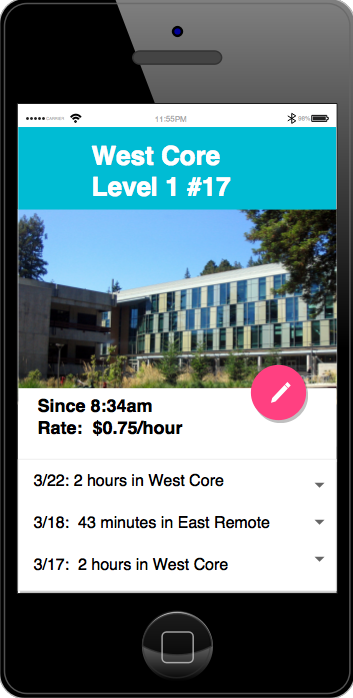
\includegraphics[width=.55\linewidth]{pictures/phone.png}
  \caption{Screen shot of the phone's redirect page to /mobile.}
%   \label{fig:3dprinted}
\end{subfigure}%
\hspace{1cm}
\begin{subfigure}{.4\textwidth}
  \centering
  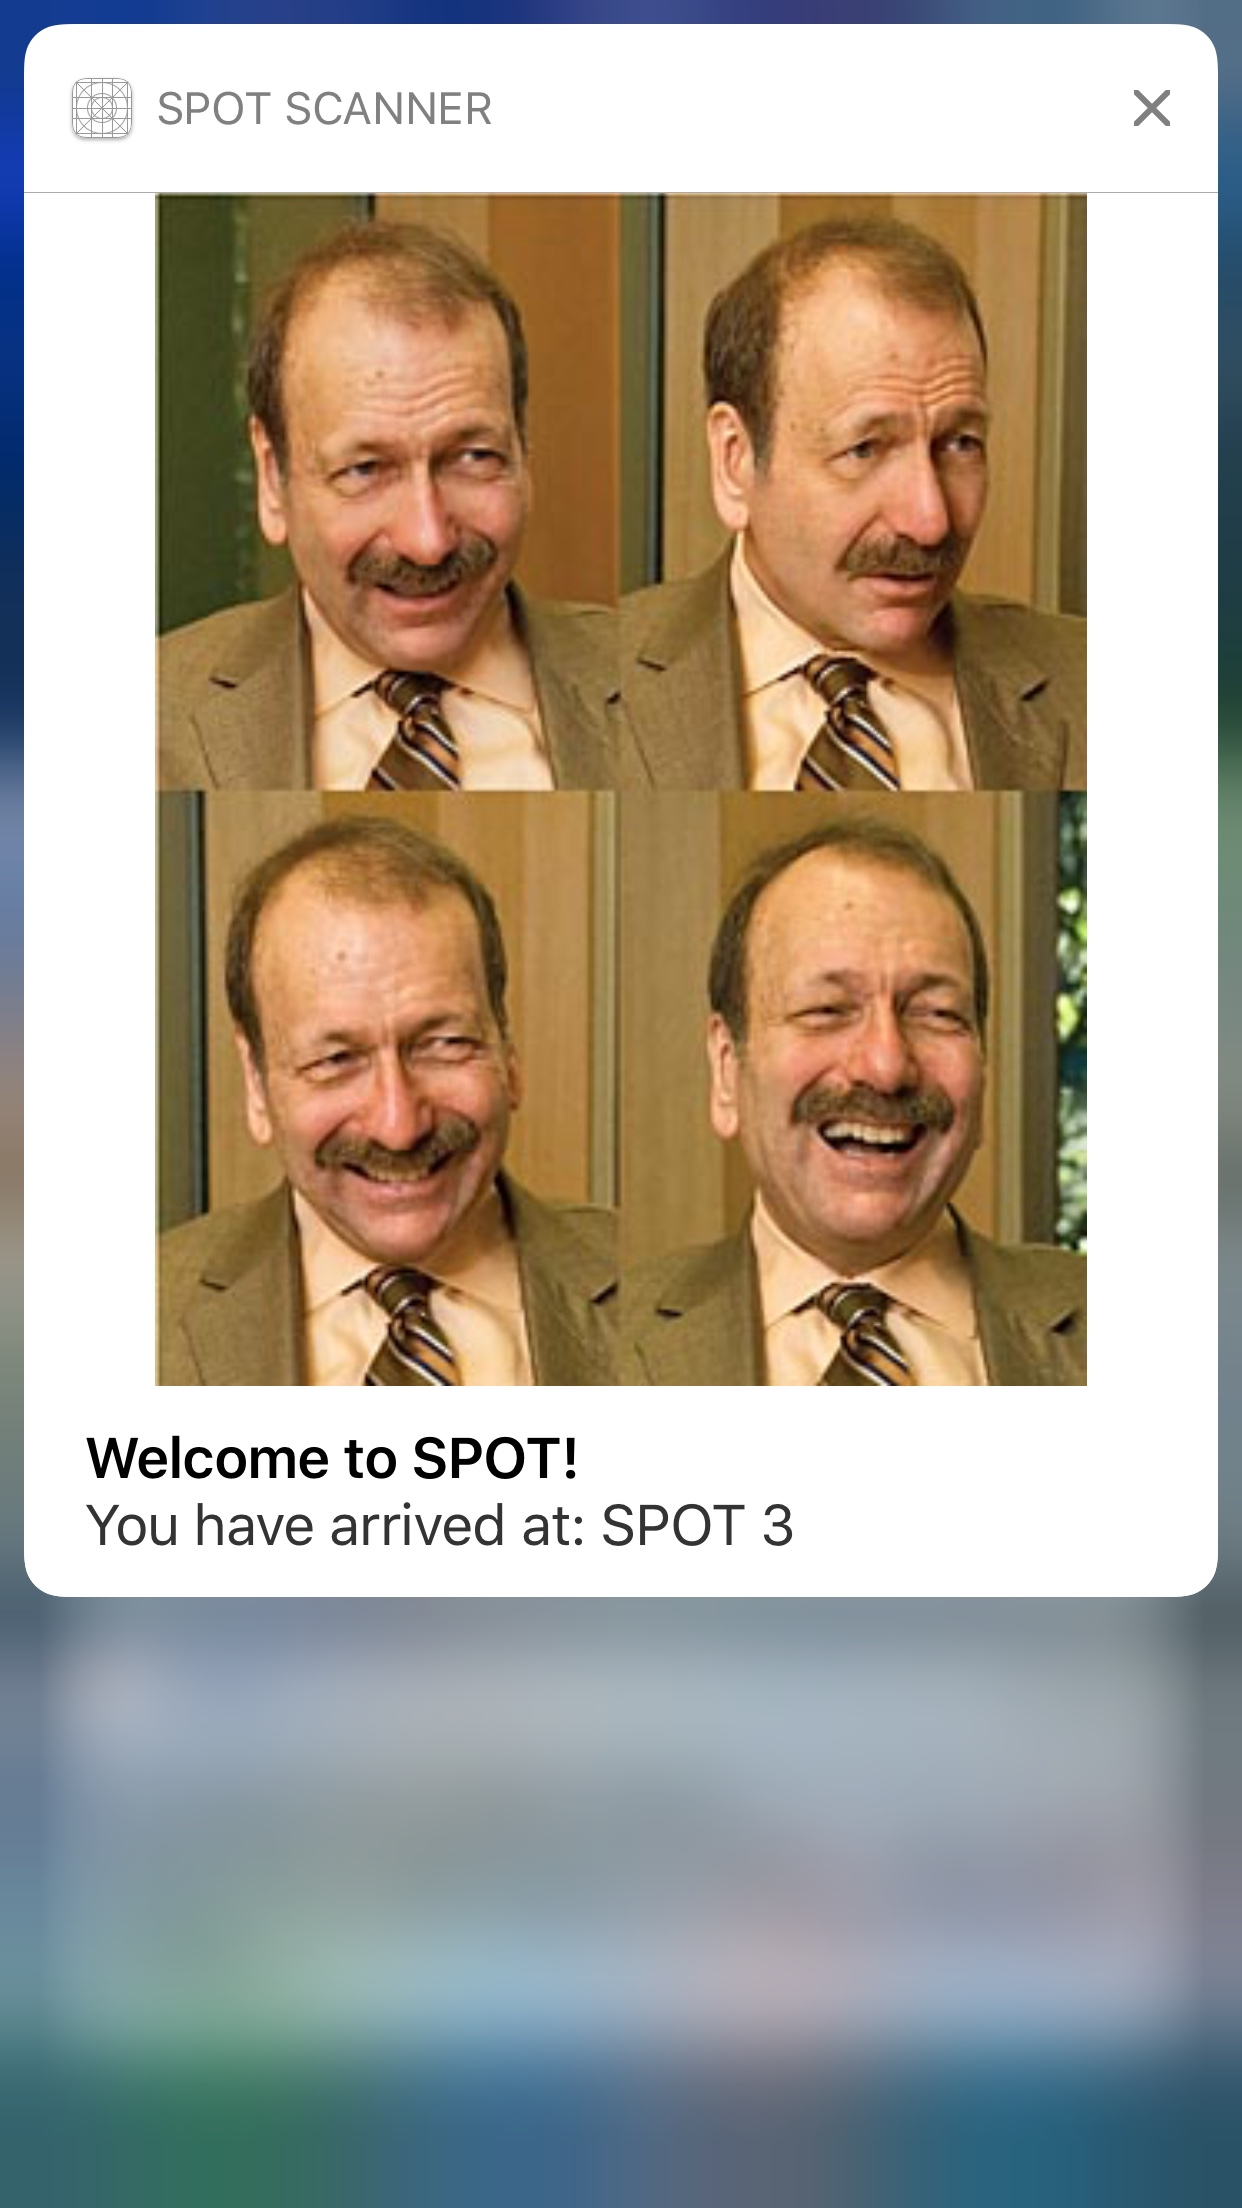
\includegraphics[width=0.6\linewidth]{pictures/blummy.jpeg}
  \caption{Screen shot of phone's notification upon arrival.}
%   \label{fig:acrylictube}
\end{subfigure}
\caption{Representation of what the driver would see on their phone.}
% \label{fig:test}
\end{figure}
%%%%%%%%%%%%%%%%%%%%%
We successfully made an Android and iOS app that was able to pick up eddystone beacons.
The app was dependent on the tutorial found from \textit{Github}\footnote{https://github.com/google/eddystone}.
Sequentially from the beacon detection, we redirected our app to our website's mobile page.
Instantaneously the server is notified that a user has arrived at a specific SPOT in our system.
To establish connection with the database, the drive must be logged in and verified by Django's authentication system.
For iOS development, you can open NSURL sessions that allows us to request verification from the server.
\begin{lstlisting}[language=C]
[[session_login dataTaskWithRequest:request_login completionHandler:
        ^(NSData *data, NSURLResponse *response, NSError *error) {
        NSString *requestReply = [[NSString alloc] initWithData:data 
                                encoding:NSASCIIStringEncoding];
        NSLog(@"requestReply_login: %@", requestReply);
}] resume];
\end{lstlisting}
Through the data received on the app, we implement a JSON parser for targeting details on what the SPOT number is as well as details such as parking rates.
% NSError *e = nil;
% NSArray *JSONarray = [NSJSONSerialization JSONObjectWithData: data options: NSJSONReadingMutableContainers error: &e];
\begin{lstlisting}[language=C]
for(int i=0;i<[JSONarray count];i++)
{
    spot_number = [[JSONarray objectAtIndex:i]objectForKey:@"number"]);
}
\end{lstlisting}
Using this sample of Objective-C we were able to implement the built in JSON parser to isolate the exact spot number correlated with the database.
With the information given from the database, the app ties the user's account with \textit{SPOT 4}, and the server stamps their arrival time immediately to automate billing.
Next, the app redirects to a URL when a beacon was detected. 
This forwards the information from the beacon to the phone, then from the phone to the cloud, from the cloud back to the phone as shown in the Figure 3. 
This is how the data is given to the cloud from the driver's phone.
With the URL that was redirected from the app, the user will eventually be able to authenticate themselves with a user login/sign up web page. 
Users can confirm the parking spot they parked in and pay through the app rather than a pay station.  


%--------------------------------------------------------------
%   CONCLUSION
%-------------------------------------------------------------
\newpage
\section{Future Work}
\subsection{Hardware}
The hardware was primarily chosen based on its ease of use and quick prototyping for quick implementation with the database.
We were focused on getting a working prototype to make sure that our idea was possible. 
We've realized that we really only need a CPU, GPU, Bluetooth transceiver, Wifi transceiver, camera, and proximity sensor. 
Using only these components we could develop our own PCB that is an optimized version of our prototype. 

It would also be beneficial if you didn't have to do a serial connection between the raspberry pi and the arduino nano. There is about a 2 second delay for the light to turn green or red which isn't the worst thing ever however it is still a little bit of an annoyance. 

The Camera software can be signficantly improved with additional image preprocessing. Currently we directly hand our images to our openALPR command. This only yields about 80\%-90\% depending on the angle. We could improve it by training the openALPR data with our own images.

\subsubsection{Power Efficient Device}
Cutting down on hardware, we can foresee a significant drop it power consumption. 
The Raspberry Pi Model 3 itself is extremely overkill and we believe that it can be marked down significantly.
Also there is an extreme amount of power that is used to power the neopixel rings. It may be best to use something else for the status light. 
For instance, we do not need all 40 GPIO pins, multi-core processors, or even all the USB ports.
Additionally, power-conserving software can be implemented to ensure our system is only at full power when absolutely necessary and remains idle or in a very low powered state normally.

\subsubsection{Magnetometer}
Currently, our ping sensor relies on sound waves. 
This requires that there is not high acoustic impedance, meaning we can't fully enclose the proximity sensor into our package. 
As discussed in the sensor section of this paper, the ping sensor relies heavily on a flat object.
For car bumpers this is not ideal since most cars are curved.
This is also undesirable since we would ideally like to weather-proof our whole design to design for longevity. 
Using other sensors, like a magnetometer, can provide a different means of sensing that can also allow for full weather-proofing of the device.
Magnetometers simplify our device to: 
'If there is a chunk of metal in front of me, signal high. 
Otherwise leave the GPIO pin low.'

\subsection{Mechanical Design}
Currently the mechanical design isn't as sturdy as we would have hoped.
We would like to one day incorporate a LCD screen into the module and find a tube that doesn't shatter as easily as acrylic. 
Also the magnets are one of the most expensive parts of the hardware. 
If possible I would recommend redesigning without them. 
It might be beneficial to also create a different sensor module that could be produced and assembled faster.
It takes approximately one full week to print all the necessary parts. 
It would also be handy to create a low cost module that doesn't have a camera but can easily detect whether or not a car is there. 
It would be nice to actually make several modules, ranging in various prices, in order to meet the needs of the potential customer.
Experimenting with a Raspberry Pi 0W would be another option too. 

\subsection{Cloud}
\begin{itemize}
    \item Refactor the sensor API to utilize DRF and JSON transactions
    \item Complete the implementation of payment methods
    \item Redesign the payment calculation algorithm as described above.
    \item Implement license plate verification
    \item Add the ability for SPOTs, sections, and lots to all define their own rates with the ability to fallthrough to the containing region
    \item Define a manager account and add checks on edit pages to make sure the user is a manager
\end{itemize}  


%--------------------------------------------------------------
%  INDEX &  BOM -- add things we bought/exact products, data sheets etc
%-------------------------------------------------------------
\newpage
\section{Index \& Bill of Materials}
% include data sheets/links to things that we bought or would like to buy in the future to further improve this project.

\begin{centering}
% Edit me. I'm preformatted
\begin{table}[!ht]\hspace{-2cm}


\centering

\resizebox{1\textwidth}{!}{\begin{tabular}{|c|c|c|c|c|}

\hline
Item Description & Price & Quantity & Subtotal & Supplier\\
\hline
Raspberry Pi 3 Starter Kit & \$50 & 4 & \$200 & Amazon\\
\hline
Raspberry Pi 3 Complete Camera Kit & \$90 & 1 & \$90 & Amazon\\
\hline
Raspberry Pi 0 Wireless Starter Kit & \$23 & 5 & \$115 & Amazon\\
\hline
Hardware mounting components (screws,nuts,bolts) & \$50 & 1 & \$10 & ACE\\
\hline
NeoPixel Ring & \$15 & 4 & \$60 & Amazon\\
\hline
Ping Sensor (HC-SR04) (Pack of 5) & \$10 & 1 & \$10 & Amazon\\
\hline
Magnetometer Sensor & \$3.50 & 5 & \$18 & Amazon\\
\hline
MicroUSB 10 pack & \$4.50 & 1 & \$5 & Amazon\\
\hline
SanDisk 8 GB SD Card & \$6 & 5 & \$30 & Amazon\\
\hline
Acrylic Tube  & \$90 & 3 & \$270 & Taps Plastic\\
\hline
\textbf{Total} & & & \textbf{\$808} &\\
\hline

\end{tabular}}
\end{table}
\end{centering}
\vspace{0.1cm}


\begin{figure}[ht]
  \caption{Pinout of the Raspberry pi 3}
  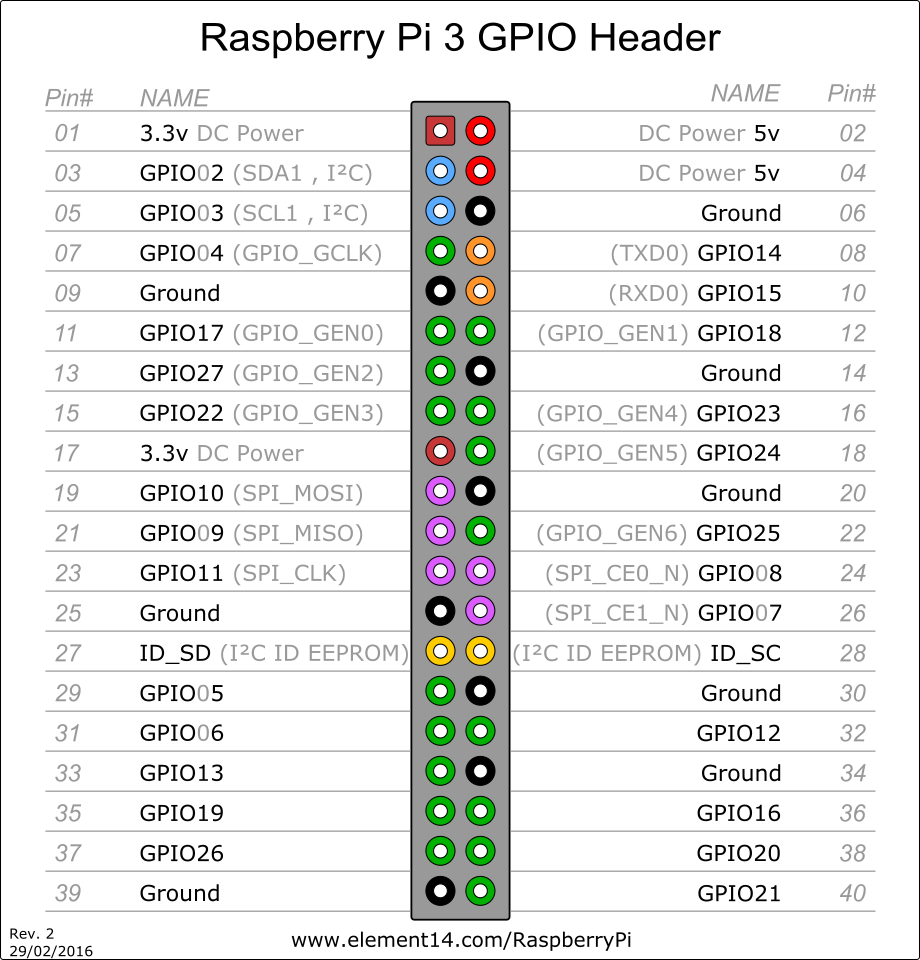
\includegraphics[width=0.7\textwidth]{pictures/pi3_gpio.png}
  \label{fig:rpi}
\end{figure}


\begin{figure}[ht]
  \caption{Pinout of the arduino nano}
  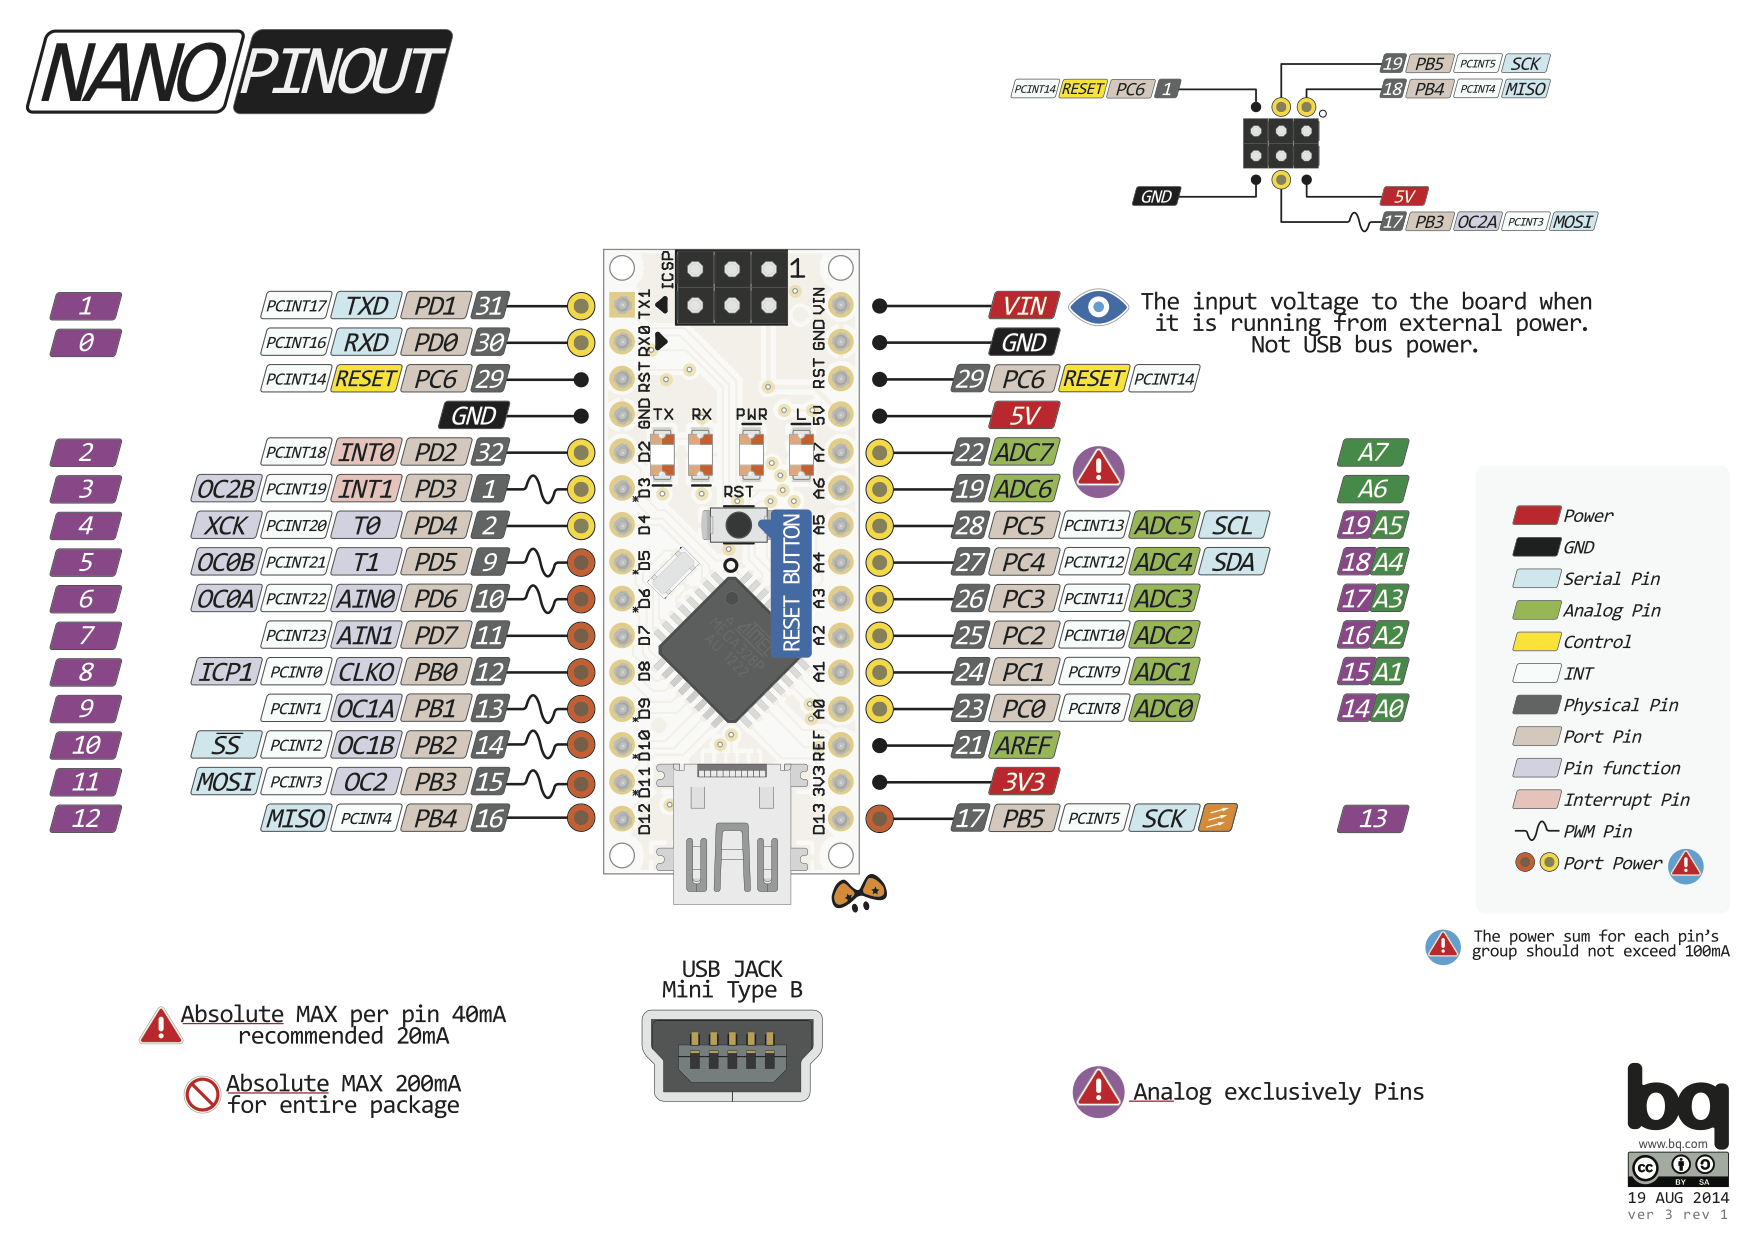
\includegraphics[width=1\textwidth]{pictures/nano.png}
\end{figure}





\end{document}